As we discussed in the previous section, our motivation is to use Theorem \ref*{thm_positive_rank} to predict points of infinite order for families of elliptic curves. However, in sections {\color{red} THE SECTIONS ON CYCLIC AND ODD} we prove that in several cases the theorem will never make such a prediction. In other words, in such cases, the product
\begin{equation}\label{eqn_localprod}
    \frac{\prod_i C_{E/F_i}}{\prod_j C_{E/F_j'}}
\end{equation}
is always a norm for every subfield $\QQ(\sqrt{D})\subseteq\QQ(\rho)$. The aim of this section is to introduce useful notation and important results that will be used throughout in the next sections, where the main results of the document are proven. 

\subsection{Notation and Preliminary Results}

In previous sections, we have discussed the behaviour of Tamagawa numbers of elliptic curves that allows us to compute them over finite extensions of number fields. The following result will be helpful to compute the local terms arising from the minimal differential in explicit examples.

    \begin{lemma}\label{lem_Dterms}
        Let $E$ be an elliptic curve over a number field $K$, $F/K$ a finite extension. Let $\pp$ be a prime in $K$ and $\fP$ a prime in $F$ above $\pp$. Let $q$ be the size of the residue field of $K$ at $\fp$. %Denote by $e_{\fP \mid \fp}$, $f_{\fP \mid \fp}$ the ramification index and residue degree of $F_{\fP} / K_{\fp}$. 

        Let $\Delta_\pp$, $\omega_{\pp}$ and $\Delta_\fP$, $\omega_{\fP}$ be the minimal discriminants and differentials for $E/K_\pp$ and $E/F_\fP$, respectively. Then the following holds.
        \begin{enumerate}[(i)]
            \setlength\itemsep{0em}
            \item If $\pp$ is unramified at $F/K$ or if $E$ has good or multiplicative reduction at $\pp$, then the minimal model of $E / K_{\fp}$ and $E / F_{\fP}$ coincide so $| \omega_{\fp} / \omega_{\fP} |_{\fP} = 1$. 
            
            \item If the residual characteristic is distinct from $2$ or $3$, and $E$ has potentially good reduction, then $v_\pp(\Delta_\pp)<12$ and the same holds for $\fP$. In particular, 
            $$\left|\frac{\omega_{\fp}}{\omega_{\fP}}\right|_{\fP} = q^{f_{\fP \mid \fp}\cdot\floor{\frac{e_{\fP\mid\fp}\nu_\fp(\Delta_\fp)}{12}}}.$$
            \item If the residual characteristic is distinct from $2$ or $3$, and $E / K_{\fp}$ has potentially multiplicative reduction then 
            $$ \left|\frac{\omega_{\fp}}{\omega_{\fP}}\right|_{\fP} = q^{f_{\fP \mid \fp} \cdot \floor{\frac{e_{\fP \mid \fp}}{2}}}.$$
        \end{enumerate}
    \end{lemma}

\begin{proof}[Proof Sketch]
    Let $e = e_{\fP \mid \fp}$, $f = f_{\fP \mid \fp}$, $\delta = v_{\fp}(\Delta_{\fp})$ and $\delta_{\fP} = v_{\fP}(\Delta_{\fP})$. Then $v_{\fP}(\Delta_{\fp}) = e n$. Thus $|\Delta_{\fp} / \Delta_{\fP} |_{\fP} = q^{f\cdot (\delta \cdot e - \delta_{\fP})}$, whence $$\left| \frac{\omega_{\fp}}{\omega_{\fP}}\right|_{\fP} = q^{f \cdot \floor{\frac{\delta \cdot e - \delta_{\fP}}{12}}}.$$ 
    \begin{enumerate}[(i)]
        \setlength\itemsep{0em}
        \setcounter{enumi}{1}
        \item If $E / K_{\fp}$ has potentially good reduction then $\delta \in \{ 2,3,4,6,8,9,10 \}$ and $\delta_{\fP} \leq 12$. By reducing to minimal Weierstrass equation for $E / F_{\fP}$ it follows that $\delta_{\fP} = \delta\cdot e - 12 \cdot \floor{\delta\cdot e / 12}$.
        
        \item Let $E / K_p$ have Kodaira type $\I_n^*$, so $\delta = 6 + n$. If $e$ is even then $E / F_{\fP}$ has Kodaira type $\I_{en}$, so $\delta_{\fP} = en$ and $\delta \cdot e - \delta_{\fP} = 6 e$.
        Else if $e$ is odd, $E / F_{\fP}$ has Kodaira type $\I_{en}^*$ so $\delta_{\fP} = 6 + en$ and $\delta\cdot e - \delta_{\fP} = 6 e - 6$. But then $\floor{(6e - 6)/12} = \floor{(e - 1)/2} = \floor{e / 2}$ since $e$ is odd.
    \end{enumerate}
\end{proof}

Now we extend the notation introduced in Notation \ref{not_contr} by defining functions on $\B(G)$. 

\begin{defn}\label{not_contr_fns}
    If $G = \Gal(F / K)$ then for $\fp \in \bQ$ we define functions $T_{\fP \mid \fp}$, $D_{\fP \mid \fp}$ and $C_{\fP \mid \fp}$ on $\B(G)$ by 
    \[ T_{\fP \mid \fp}(H) = T_{\fP \mid \fp}(E / F^H), \quad D_{\fP \mid \fp}(H) = D_{\fP \mid \fp}(E / F^H), \quad C_{\fP \mid \fp}(H) = C_{\fP \mid \fp}(E / F^H), \]
    as defined in Notation \ref{not_contr}.
    Note that if $H$, $H'$ are conjugate then $F^H$, $F^{H'}$ are isomorphic, and so the values of these functions are constant on conjugate subgroups, hence they are well-defined. When $K = \bQ$ we write $p$ instead of $\fp$. Define $C \colon \B(G) \to \bQ^{\times}$ by $C \colon H \mapsto C_{E / F^H}$.  
\end{defn}
 
{\color{red} EHHHH maybe I need to change some of this to be more general}
Note that $C_{\fP \mid p}$ is a $D_p$-local function. Indeed, suppose $D_p = \Gal(F_w / \bQ_p)$, where $F_w$ denotes the completion of $F$ with respect to a place $w$ lying above $p$. For a number field $K$ and place $v$, define $$C_v(E / K) = c_v(E / K) \cdot \left| \omega / \omega_v^{\min} \right|_v.$$ We use the same notation if $K$ is a local field (then the $v$ subscript holds no meaning).
One has
\begin{equation*}
    C_{\fP \mid p} = (D_p, C_v)
\end{equation*}
where $C_v$ is a function on $\B(D_p)$ sending $H \mapsto C_v(E / F_w^H)$.

The following proposition describes these functions in the language introduced in Section \ref{sec-norm-rels} for each reduction type of $E / \bQ$. We do not attempt to write a formula for $T_{\fP \mid p}$ in the case of additive reduction, computing this involves using Lemma \ref{lem_add_tam}.

\begin{prop}\label{prop_local_fns}
    Let $E / \bQ$ be an elliptic curve, $G = \Gal(F / \bQ)$ and $p$ a prime of $\bQ$. Let $n = v_p(\Delta_E)$. Consider the functions $C_{\fP \mid p}$, $T_{\fP \mid p}$, and $D_{\fP \mid p}$ on $\B(G)$ defined above. Then,
    \begin{enumerate}[(i)]
        \setlength\itemsep{0em}
        \item If $E / \bQ_p$ has good reduction, $C_{\fP \mid p} = 1$,
        \item If $E / \bQ_p$ has split multiplicative reduction then $C_{\fP \mid p} = T_{\fP \mid p} = (D_p, I_p, e n)$,
        \item If $E / \bQ_p$ has non-split multiplicative reduction, 
        $C_{\fP \mid p} = T_{\fP \mid p} = \left(D_p, I_p,
        \left\{\begin{smallmatrix}
            2   & 2 \mid en, 2 \nmid f,  \\
            en   &  2 \mid f, \\
            1   & \text{else}
        \end{smallmatrix}\right.\right),$ 
        \item If $E / \bQ_p$ has potentially good reduction and $p \not= 2, 3$, $D_{\fP \mid p} = (D_p, I_p, p^{f \floor{e n /12}})$, 
        \item If $E / \bQ_p$ has potentially multiplicative reduction and $p \not= 2, 3$, $D_{\fP \mid p} = (D_p, I_p, p^{f \floor{e / 2}})$.
    \end{enumerate}  
\end{prop} 
 
\begin{proof}
    \
    \begin{enumerate}[(i)]
        \setlength\itemsep{0em}
        \item Clear. 
        \item Lemma \ref{lem_Dterms}(i) implies $D_{\fP \mid p} = 1$. If $K' / \bQ_p$ is a finite extension of ramification degree $e$, then $E / K'$ has split multiplicative reduction of type $\I_{en}$, which has Tamagawa number $en$ by Lemma \ref{lem_mult_tam}.
        \item As for split, $D_{\fP \mid p} = 1$. The description follows from applying Proposition \ref{prop_semi_red} (iii) (non-split becomes split when the residue degree is even), and Lemma \ref{lem_mult_tam}. 
        \item Follows from Lemma \ref{lem_Dterms}(ii),
        \item Follows from Lemma \ref{lem_Dterms}(iii).
    \end{enumerate}
\end{proof}
%An immediate consequence of this notation is the fact that 
%$$C_{E/F}=\prod_{\pp}C_{\mathfrak{P}\mid \pp}(F/K);$$
%that is, we can calculate $C_{E/F}$ by calculating the contribution locally at each prime of $K$. 
%{\color{red} also important to mention at some point that if the reduction is semistable, then the terms in a norm relation coming from the discriminant also vanish. Probably this would have to be introduced later.}

\begin{rem}\label{rephrase-thm}
    We rephrase Theorem \ref{thm_positive_rank} in the language introduced in $\S$\ref{sec-norm-rels}. 
    Replacing $\rho$ by the sum of its conjugates by elements of $ \Gal(\bQ(\rho) / \bQ(\sqrt{D}))$, we may assume that $\bQ(\rho) = \bQ(\sqrt{D})$. Note that this does not affect the order of $\rho$ in $\C(G)$, nor the set of $\rho$-relations (since $\repnorm{\rho}$ is unchanged). 
    
    Let $\Theta$ be a $\rho$-relation with $\bC[G / \Theta] = \repnorm{\rho}^{\oplus m}$. Let $C \colon \B(G) \to \bQ^{\times}$ be the function sending $H \mapsto C_{E / F^H}$. The theorem then states that, if $\Theta$ is not a norm relation for $C$ when $m$ is odd, or if $C(\Theta) \not\in (\bQ^{\times})^2$ for $m$ even, then $ \rk E / F > 0$. 
\end{rem}

\subsection{Number Theoretic Results}

In the following sections, we will also require some number theoretic results, and we state and prove them in this subsection. At the end, we also prove two surprising and technical consequences of these results on Type II and $\mathrm{II^*}$ elliptic curves. The first result is more classical, and it explicitly describes the quadratic subfields of cyclotomic fields $\QQ(\zeta_d)$ where at most one odd prime factor $q$ divides $d$.

\begin{lemma}\label{lem_subfields}
    Let $q$ be an odd rational prime, $n,m$ a positive integers and let $q^*=(-1)^{(q-1)/2}q$. Then the following holds.

    \begin{table}[!ht]
        \centering
        \begin{tabular}{|l|l|l|}
        \hline
        Cyclotomic field                    & Conditions & Quadratic subfields                   \\ \hline
        $\QQ(\zeta_{q^n})$                  & any $n$    & $\QQ(\sqrt{q^*})$            \\ \hline
        \multirow{3}{*}{$\QQ(\zeta_{2^m})$} & $m=1$      & none                                  \\ \cline{2-3} 
                                            & $m=2$      & $\QQ(i)$                              \\ \cline{2-3} 
                                            & $m\geq3$   & $\QQ(i),\QQ(\sqrt{2}),\QQ(\sqrt{-2})$ \\ \hline
        \multirow{3}{*}{$\QQ(\zeta_{2^mq^n})$}  & $m=1$, any $n$      & $\QQ(\sqrt{q^*})$     \\ \cline{2-3} 
                                            & $m=2$, any $n$      & $\QQ(i),\QQ(\sqrt{q}),\QQ(\sqrt{-q})$                              \\ \cline{2-3}
                                            & $m\geq 3$, any $n$      & $\QQ(i),\QQ(\sqrt{2}),\QQ(\sqrt{-2}),\QQ(\sqrt{q}),\QQ(\sqrt{-q}),\QQ(\sqrt{2q}),\QQ(\sqrt{-2q})$                              \\ 
                                             \hline
        \end{tabular}
        \end{table}

\end{lemma}

\begin{proof}
    Firstly, we remark that the discriminant of the field $\QQ(\sqrt{D})$, with $D$ squarefree is
    \begin{equation}
        \Delta(\QQ(\sqrt{D}))=
        \begin{cases}
            D \ \quad\text{  if } D\equiv1\pmod{4},\\
            4D \quad\text{ if } D\equiv2,3\pmod{4}.
        \end{cases}
    \end{equation}
    In addition, we also recall that $\QQ(\zeta_N)/\QQ$ is a Galois extension with $\Gal(\QQ(\zeta_N)/\QQ)=(\ZZ/N\ZZ)^*$ and that a rational prime $r$ ramifies in $\QQ(\zeta_N)/\QQ$ if and only if $r\mid N$. The result follows by combining these two properties with the Galois correspondence, as we show now.

    If $q$ is odd, then $\Gal(\QQ(\zeta_{q^n})/\QQ)=(\ZZ/q^n\ZZ)^*=C_{q^{n-1}(q-1)}$ is a cyclic group of even order, and therefore $\QQ(\zeta_{q^n})$ has one unique quadratic subfield, which can only ramifiy at $q$. If $q\equiv1\pmod{4}$, then the only such field is $\QQ(\sqrt{q})$ and if $q\equiv3\pmod{4}$ the only such field is $\QQ(\sqrt{-q})$. This proves the first row. 

    Since $\QQ(\zeta_2)=\QQ$ and $\QQ(\zeta_4)=\QQ(i)$, the second and third row are immediate. For $m\geq3$, $\Gal(\QQ(\zeta_{2^m})/\QQ)=(\ZZ/2^m\ZZ)^*=C_2\times C_2^{m-2}$ and therefore $\QQ(\zeta_{2^m})$ has three quadratic subfields that can only ramify at $2$. Again, it is easy to check that the only such fields are $\QQ(i)$, $\QQ(\sqrt{2})$ and $\QQ(\sqrt{-2})$, as desired. Alternatively, one can also show that $\zeta_8=(1+i)/\sqrt{2}$, which also implies the result. This proves the third row.

    The remaining rows are essentially a combination of the results we have already shown. We note that $\Gal(\QQ(\zeta_{2q^n})/\QQ)=(\ZZ/2q^n\ZZ)^*$ is cyclic while 
    $$\Gal(\QQ(\zeta_{2^mq^n})/\QQ)=(\ZZ/2^mq^n\ZZ)^*=(\ZZ/2^m)^*\times(\ZZ/q^n\ZZ)^*=C_2\times C_{2^{m-2}}\times C_{p^{n-1}(p-1)}.$$
    Hence, $\QQ(\zeta_{2^mp^n})$ has one unique quadratic subfield if $m=1$ which must be $\QQ(\sqrt{p^*})$, three quadratic subfields if $m=2$, which must be $\QQ(i),\QQ(\sqrt{p}),\QQ(\sqrt{-p})$, and seven quadratic subfields if $m\geq 3$. Since $\QQ(\zeta_8),\QQ(\zeta_q)\subseteq\QQ(\zeta_{2^mq^n})$, it follows that $\QQ(\sqrt{D})\subseteq\QQ(\zeta_{2^mq^n})$ for $D\in\{-1,\pm2,\pm q,\pm 2q\}$. These are seven distinct quadratic fields, so we are done.
\end{proof}

The following two results are naturally phrased in terms of local fields. The first gives a necessary divisibility condition on primes ramifying in finite extensions of number fields.

\begin{prop}\label{prop_totally_ramified}
    Let $F/\QQ_p$ be a finite extension with residue field $\kappa$. Then there exists a tame, totally ramified cyclic extension $F_n$ of degree $n$ over $F$ if and only if $n\mid|\kappa^*|$.
\end{prop}

\begin{proof}
    Assume first that $n\mid|\kappa^*|$. Let $\pi$ be a normalizer of $F$ and consider $F_n=F(\pi^{1/n})$. We claim that $F_n$ satisfies the desired properties. Since $n\mid|\kappa^*|$, $\kappa$ contains all $n$-th roots of unity and therefore the polynomial $x^n-1$ factors into linear terms in $\kappa[x]$. The divisibility condition above implies $\Char\kappa\nmid n$ and hence by Hensel's Lemma $x^n-1$ also factors into linear terms in $F[x]$. In other words, $\QQ_p(\zeta_n)\subseteq F$ and therefore $F_n$ is the splitting field of the polynomial $x^n-\pi$. This shows that $F_n/F$ is a tame, totally ramified Galois extension, and the map 
    \begin{align*}
        \psi: \Gal(F_n/F)&\longrightarrow \mu_n\cong C_n\\
        \sigma &\longmapsto \frac{\sigma(\pi^{1/n})}{\pi^{1/n}}
    \end{align*}
    is an isomorphism of groups, which proves that the extension is cyclic of degree $n$.

    Conversely, suppose that $F_n/F$ is a tame, totally ramified cyclic extension of degree $n$. Any such field extension is generated by the $n$-th root of some uniformizer $\pi$ of $F$ (see \cite[Theorem 11.10]{Sun1}), and therefore $F_n=F(\pi^{1/n})$. The polynomial $x^n-\pi$ is Einstein over $F$, and therefore irreducible over $F$. Since $F_n/F$ is assumed to be Galois, all roots of $x^n-\pi$ lie in $F_n$. In particular, $\QQ(\zeta_n)\subseteq F_n$. Since $\Char\kappa\nmid n$, it follows that $\kappa$ also contains all $n$-th roots of unity, proving that $n\mid|\kappa^*|$ as desired. 
\end{proof}

The second result is more technical and specific, but has interesting consequences on elliptic curves. 

\begin{lemma}\label{lem_localC4}
    Let $F/K$ be a finite Galois extension of local fields of characteristic $0$ with residual characteristic distinct from $2$ or $3$ and such that $\Gal(F/K)=C_4$. If the ramification index and residual degree are both $2$, then $F=K(\sqrt{u},\sqrt{v\pi})$ where $\pi$ is a uniformizer of $K$, $u$ is a non-square unit of $K$ and $v$ is a non-square unit of $K(\sqrt{u})$.
    In particular, if $\varpi$ is a uniformizer of $F$, then $\varpi^2/\pi$ is a non-square unit of $F$.
\end{lemma}

\begin{proof}
    %We first recall a fundamental property of local fields. If $K$ is any local field of characteristic $0$ and residual characteristic distinct from $2$, then $K$ has three quadratic extensions, two of which are ramified and one unramified. 
    Let $L=F^{C_2}$ be the unique intermediate field of $F/K$. Since $F$ is also the fixed field by intertia, then $F/L$ is ramified while $L/K$ is unramified. We recall that $K$ has a unique unramified extension of any degree, and the unramified quadratic extension is generated by any $\sqrt{u}$ of any non-square unit of $K$. Hence $L=K(\sqrt{u})$ for some non-square unit, and note that $\pi$ is a uniformizer of $L$ too. Since $F/L$ is ramified, $F$ is either generated by $\sqrt{\pi}$ or $\sqrt{v\pi}$ for some non-square unit $v$ of $L$. If $F=L(\sqrt{\pi})$, then $F$ contains all three quadratic extensions of $K$, in which case $\Gal(F/K)=C_2\times C_2$, a contradiction. Hence, necessarily, $F=L(\sqrt{v\pi})=K(\sqrt{u},\sqrt{v\pi})$ for some non-square unit $v$ of $L$.

    To prove the last statement, note that $\sqrt{v\pi}$ is a uniformizer of $F$ and $(\sqrt{v\pi})^2/\pi=v$ is a non-square unit of $F$. Since any two uniformizers are equal up to multiplication by units, the result follows. 
\end{proof}

We now prove two technical consequences of these results about the behaviour of Type II or $\mathrm{II}^*$ elliptic curves over local fields $K$. We advise the reader to skip the proofs by now and revisit them when these results are used later.

\begin{lemma}\label{lem_nottwo}
    Let $p\geq 5$ be a rational prime and $F_\fP/K_\fp/\QQ_p$ be finite extensions with $F_\fP/K_\fp$ Galois, ramified and $\Gal(F_\fP/K_\fp)=C_3$. Let $$E/\QQ_p:y^2=x^3+Ax+B$$ be a minimal Weierstrass equation at $\pp$ with potentially good reduction. Let $n=\nu_\pp(\Delta)$ be the valuation of the minimal discriminant. If $\gcd(n,12)=2$, then $\sqrt{\Delta}\in K_\pp$.
\end{lemma}

\begin{proof}
    The condition that $E$ has additive reduction is equivalent to $A,B\in\pp$, and the condition on ramification implies that $3\mid N(\pp)-1$ by Proposition \ref{prop_totally_ramified}. In addition, by Lemma \ref{lem_Dterms}(b), we know that $\nu_\pp(\Delta)<12$, so we need to consider two cases: $n=2$ and $n=10$, and we consider them separately. By Hensel's Lemma, $\sqrt{\Delta}\in K_\pp$ is equivalent to $\sqrt{\Delta}\in \kappa_\pp$ where $\kappa_\pp$ is the residue field of $K_\pp$. Recall that when $E$ has this simple expression, $\Delta=-16(4A^3+27B^2)$.


    \textbf{Case $n=2$:}

    In this case, $\nu_\pp(-4A^3-27B^2)=2$ and this implies that $\nu_\pp(B)=1$. Note that we also have that $A,B\in p\ZZ_p$ and therefore $\nu_p(B)=1$ and $\nu_p(-4A^3-27B^2)=2$. Let $\FF_p=\ZZ_p/p\ZZ_p$ be the residue field of $\QQ_p$. Then 
    $$\frac{-4A^3-27B^2}{p^2}\equiv -3\left(\frac{3B}{p}\right)^2\pmod{p},$$
    and hence $\sqrt{\Delta}\in\FF_p$ if and only if $\sqrt{-3}\in K_\pp$. 
    If $p\equiv1\pmod{3}$, then
    $$\left(\frac{-3}{p}\right)=\left(\frac{p}{3}\right)=1,$$
    and hence $\sqrt{\Delta}\in \FF_p\subseteq \kappa_\pp$. If $p\equiv 2\pmod{3}$, then from the condition that $3\mid N(\pp)-1$, it follows that the extension $\kappa_\pp/\FF_p$ has even degree. By the uniqueness of extensions of finite fields, it follows that $\sqrt{\Delta}\pmod{\pp}\in\kappa_\pp$ as desired.

    \textbf{Case $n=10$:} 

    In this case, $\nu_\pp(-4A^3-27B^2)=10$. When $E$ is defined by this simple expression, then $c_4=-48A$ and since $E$ is assumed to have potentially good reduction, $\nu_\pp(j)=\nu_\pp(A^3/\Delta)=3\nu_\pp(A)-10\geq 0$. Hence, $\nu_\pp(A^3)\geq12$ which implies that $\nu_\pp(-27B^2)=10$ or, equivalently, that $\nu_\pp(B)=5$. This means that $\nu_p(B)=5$ if $K_\pp/\QQ_p$ is unramified or $\nu_p(B)=1$ if $K_\pp/\QQ_p$ has ramification index $2$. In the latter case, we have that $v_p(4A^3+27B^2)=2$ and we are back to the case $n=2$. So assume that $K_\pp/\QQ_p$ is unramified. Then
    $$\frac{-4A^3-27B^2}{p^{10}}\equiv -3\left(\frac{3B}{p^5}\right)^2\pmod{p},$$
    and therefore $\sqrt{\Delta}\in\FF_p$ if and only if $\sqrt{-3}\in K_\pp$. The remaining of the proof is identical to the case $n=2$.
\end{proof}

\begin{lemma}\label{lem_notthree}
    Let $p\geq 5$ be a rational prime and $F_\fP/K_\fp/\QQ_p$ be finite extensions with $F_\fP/K_\fp$ Galois, $\Gal(F_\fP/K_\fp)=C_4$ and ramification index and residual degree equal to $2$. Let $$E/\QQ_p:y^2=x^3+Ax+B$$ be a minimal Weierstrass equation at $\pp$ with potentially good reduction. Let $n=\nu_\pp(\Delta)$ be the valuation of the minimal discriminant. If $\gcd(n,12)=2$, then $\sqrt{B}\not\in F_\fP$.
\end{lemma}

\begin{proof}
    By Lemma \ref{lem_localC4}, we know that $F_\fP=K_\pp(\sqrt{u},\sqrt{v\pi})$ where $\pi$ is a uniformizer of $K$, $u$ is a non-square unit of $K$ and $v$ is a non-square unit of $K(\sqrt{u})$. We also note that $\pi$ is a uniformizer of $K(\sqrt{u})$.
    Similarly to the previous proof, we need to consider the case $n=2$ and $n=10$. 

    \textbf{Case $n=2$:}

    In this case, $\nu_\pp(B)=1$ and therefore $B=\mu\pi$ for some unit $\mu$ of $K$. Since the extension $K(\sqrt{u})/K$ is unramified of degree $2$, $\mu=\lambda^2$ for some unit $\lambda$ of $K(\sqrt{u})$. Therefore, if $\varpi$ is a uniformizer of $F_\fP$, then $B/\varpi^2=\lambda^2\pi/\varpi^2$ is a non-square unit by Lemma \ref{lem_localC4}. In particular, $\sqrt{B}\not\in F_\fP$.

    \textbf{Case $n=10$:}
    This case is solved similarly. Following the same argument as in Lemma \ref{lem_nottwo}, it follows that $\nu_\pp(B)=5$ and hence $B=\mu\pi^5$ where $\mu$ is a unit in $K$ and $\mu=\lambda^2$ for some unit $\lambda$ in $K(\sqrt{u})$. Hence,
    $$\frac{B}{\varpi^{10}}=\frac{\lambda^2\pi^5}{\varpi^{10}}=\left(\frac{\lambda\pi^2}{\varpi^4}\right)^2\frac{\pi}{\varpi^2}$$
    is a non-square unit of $F_\fP$, which implies that $\sqrt{B}\not\in F_\fP$.
\end{proof}

\subsection{Cyclic Extensions}

The aim of this subsection is to give a complete analysis of the case when $F/K$ is a cyclic extension of number fields. We show that for any $d\geq 2$ and representation $\rho$ of $C_d$, the product \eqref{eqn_localprod} of local factors is the norm of any quadratic subfield of $\QQ(\rho)$. 
%We also provide an exhaustive list of cases when the product may not be a norm of quadratic subfield of $\QQ(\rho)$. 
Firstly, we recall the following result, whose proof was covered in Example \ref{cyclic-relns}.

\begin{lemma}\label{lem_relation}
    Let $\rho$ be a representation of the cyclic group $C_d$. Then there is one unique relation $\Theta_\rho\in B(C_d)$ such that 
    $$\CC[C_d/\Theta_{\rho}]=\repnorm{\rho}=\bigoplus_{\fg\in\Gal(\QQ(\rho)/\QQ)}\rho^{\fg}.$$
    In particular, if $\rho=\psi_d$ is a faithful character of $C_d$, then
    $$\Theta_{\psi_d}=\sum_{k\mid d}\mu(k)C_k.$$
\end{lemma}


%We also the following definition that characterises those $d$ that always give norms of the quadratic subfields and those that do not. Recall that given some integer $d\geq 2$, $\rad(d)=\prod_{p\mid d}p$ is the smallest squarefree integer dividing $d$.

%\begin{defn}
    %Let $d\geq 2$ be an integer. We say that $d$ is \textbf{bad} if either $\rad(d)=2$ or $\rad(d)=6$ and $4\mid d$. Otherwise, we say that $d$ is \textbf{good}.
%\end{defn}

The main result of this section is to prove that for any $d$ and any representation $\rho$ od $C_d$, the product of local factors of an elliptic curve over $\QQ$ always gives a norm of any quadratic subfield of $\QQ(\rho)$.

\begin{thm}\label{thm_consistent_cyclic}
    Let $d\geq2$ be a positive integer and let $F/K$ be a Galois extension of number fields such that $\Gal(F/K)=C_d$. Let $\rho$ be a representation of $C_d$ and let $\Theta_\rho\in B(C_d)$ be such that
    $$\CC[G/\Theta_\rho]=\repnorm{\rho}.$$

    If $E/\QQ$ is a semistable elliptic curve at $2$ and $3$, then for any $\QQ(\sqrt{D})\subseteq\QQ(\rho)$,
    $$C(\Theta_\rho)\in N_{\QQ(\sqrt{D})/\QQ}(\QQ(\sqrt{D})^{\times}).$$
\end{thm}

The first step towards proving this theorem is to show that if the theorem holds for faithful characters, then it holds for arbitrary representations. 

\begin{lemma}
    Suppose that Theorem \ref{thm_consistent_cyclic} holds for faithful characters $\psi_d$. Then it also holds for any representation $\rho$ of $C_d$.
\end{lemma}
\begin{proof}
    Firstly, we show that the theorem also holds for arbitrary characters of $C_d$. Let $\psi_{d'}$ be a character of $C_d$ of order $d'$ for some $d'\mid d$, and recall that 
    $$\Theta_{\psi_{d'}}=\sum_{k\mid d'}\mu(k)C_{dk/d'}.$$ Since $\ker\psi_{d'}=C_{d/d'}$, we can view $\psi_{d'}$ as a faithful character of $C_{d'}$. Then the result follows immediately from the theorem applied to ${d'}$ and the $C_{d'}$-extension $F/F^{C_{d'}}$.
    Now assume that $\rho$ is any representation of $C_d$. Then $\repnorm{\rho}$ is a rational valued representation, and the representations
    $$\chi_k:=\repnorm{\psi_k}$$
    for each $k\mid d$ are a basis of the rational representations. Hence, there is a unique decomposition
    $$\repnorm{\rho}=\sum_{k\mid d}a_k\chi_k,\ a_k\in\ZZ,$$
    where
    which in particular implies that 
    $$C(\Theta_\rho)=\prod_{k\mid d}C(\Theta_{\psi_k})^{a_k}\equiv \prod_{\substack{k\mid d \\ a_k\text{ odd}} }C(\Theta_{\psi_k})^{a_k}\pmod{\QQss}.$$
    In Proposition \ref{index-fn-trivial} we showed that if $\QQ(\rho)\nsubseteq \QQ(\zeta_d)=\QQ(\psi_k)$, then $a_k$ was even, so if $a_k$ is odd, then $\QQ(\rho)\subseteq\QQ(\zeta_k)$. If $\QQ(\sqrt{D})$ is a quadratic subfield of $\QQ(\rho)$, then $C(\Theta_{\psi_k})$ is a norm from $\QQ(\sqrt{D})$ whenever $a_k$ is odd. This implies that $C(\Theta_\rho)$ is a norm from $\QQ(\sqrt{D})$ too, and thus Theorem \ref{thm_consistent_cyclic} holds.
\end{proof}

This lemma has the great advantage that it allows us to restrict our attention to faithful characters of $C_d$. To simplify notatation, we will denote $\Theta_d=\sum_{k\mid d}\mu(k)C_k\in B(C_d)$ as the $\psi_d$-relation, where $\psi_d$ is a faithful character of $C_d$.

\begin{rem}\label{rem_radical}
    Lemma \ref{lem_relation} has an important consequence. Given an integer $d\geq2$, note that a subgroup $C_k$ appears in $\Theta_d$ if and only if $C_k\leq C_{\rad(d)}$. Consequently, in terms of fields, if $L_k=F^{C_{d/k}}$ is the unique intermediate field with $[L_k:\QQ]=k$ for each $k\mid d$, then $C(\Theta_d)$ contains the local factors of $L_k$ if and only if $L_{d/\rad(d)}\subseteq L_k\subseteq F$.

    Following this observation, we will compute $T(\Theta_d)$ and $D(\Theta_d)$ by computing locally $\Tp(\Theta_d)$ and $\Tp(\Theta_d)$ for each prime $\pp$ of some conveniently chosen subfield $L_k\subseteq L_{d/\rad(d)}$, and then combinining this local information via the formula
    \begin{equation}\label{eqn_local_contr}
        T(\Theta_d)=\prod_{\pp}\Tp(\Theta_d)=\prod_\pp\left(\prod_{k\mid d} \Tp(C_k)^{\mu(k)}\right),    
    \end{equation}
    and where the same equation holds for $D(\Theta_d)$.
\end{rem}

To compute $\Tp(\Theta_d)$ for multiplicative reduction, the following notation will also be useful.

\begin{notation}\label{not_n}
    Let $n$ be a positive integer. Let 
    \[
        \tilde{n}=
        \begin{cases}
            1 \text{ if } n \text{ is odd,}\\
            2 \text{ if } n \text{ is even.}
        \end{cases}
    \]
\end{notation}
Therefore, if $E$ is an elliptic curve with multiplicative reduction at some prime $\pp$ of $K$ and $n=\nu_\pp(\Delta_{E,\pp}^{\min})$, then $c_\pp(E/K)=n$ if the reduction is split and $c_\pp(E/K)=\tilde{n}$ if non-split.

We divide the proof of Theorem \ref{thm_consistent_cyclic} for faithful characters into two separate cases: odd and even cyclic extensions. The main idea in both cases is to simplify the general case into smaller cases where we can directly compute $\Cp(\Theta_d)$ for each finite place $\pp$ of $K$. Unless stated otherwise, we assume thoughout that $$\Theta_d=\sum_{k\mid d}\mu(k)C_k\in B(C_d).$$





\subsubsection{Odd Cyclic Extensions} \label{case_Cp}

For the first case, we assume that $d$ is odd. Following the observation in Remark \ref{rem_radical}, we will calculate $\Cp(\Theta_d)$ for each finite place $\pp$ of some subfield of $F^{C_{\rad(d)}}$. However, before we calculate these terms explicitly for distinct cases, we prove a technical result that considerably simplifies the calculations of $\Dp(\Theta_d)$.

\begin{lemma}
    Let $q$ be an odd prime and $L/K$ a Galois extension of number fields such that $\Gal(L/K)=C_q$, and let $\pp$ be a prime in $K$. Let $E/\QQ$ be an elliptic curve and $\Theta_q=C_1-C_q\in B(C_q)$. Then by changing the model of $E$ over $K$, and therefore by rescaling the discriminat of $E$, $\Dp(\Theta_q)$ does not change up to squares.
\end{lemma}
\begin{proof}
    Let $\Delta_E,\Delta_E'$ be the discrimiants of two models of $E$ over $K$, and let $\lambda=(\Delta_E'/\Delta_E)^{1/12}\in K$. Write $\Dp'(\Theta_q)$ and $\Dp(\Theta_q)$ for the value usual terms using $\Delta_E$ and $\Delta_E'$ as discriminants, respectively. Then a simple calculation shows that
    
    $$\Dp(\Theta_q)=\frac{\prod_{\fP\mid\fp}|\lambda|_\fP}{|\lambda|_\pp}\Dp'(\Theta_q).$$
    Hence, the result will follow by showing that $\prod_{\fP\mid\fp}|\lambda|_\fP/|\lambda|_\pp\in\QQss$. 
    
    There are three cases, depending on the splitting behaviour of $\pp$ in $F$. 
    \begin{itemize}
        \item If $\pp$ splits, then there are $q$ primes above $\pp$ with the same residue field and normalized valuation. Hence $\prod_{\fP\mid\fp}|\lambda|_\fP=|\lambda|_\pp^q$.
        \item If $\pp$ is inert, then there is one prime $\fP$ above $\pp$ whose residue field is a degree $q$ extension and with the same normalized valuation. Hence $|\lambda|_\fP=|\lambda|_\pp^q$.
        \item If $\pp$ ramifies, then there is one prime $\fP$ above $\pp$, with equal residue field but with normalized valuation satisfying $\nu_\fP(\lambda)=q\mu_\pp(\lambda)$. Hence $|\lambda|_\fP=|\lambda|_\pp^q$ too.
    \end{itemize}
    Hence, we always have that 
    $$\frac{\prod_{\fP\mid\fp}|\lambda|_\fP}{|\lambda|_\pp}=|\lambda|_\pp^{q-1}\in\QQss$$
\end{proof}

The great advantage of this result is that once a prime $\pp$ has been chosen in some subfield of $F^{C_{\rad(d)}}$, we will be able to assume that $\Delta_E=\Delta_{E,\pp}^{\min}$. 

To prove Theorem \ref{thm_consistent_cyclic} for odd $d$, we first calculate $\Cp(\Theta_d)$ for simple cases, and then we use them to prove the general case. The following lemmas build on this idea.

\begin{lemma}\label{lem_Cp}
    Let $q$ be an odd rational prime, $F/K$ a Galois extension of number fields such that $\Gal(F/K)=C_q$ and $E/\QQ$ an elliptic curve with semistable reduction at $2$ and $3$. If $\Theta_q=C_1-C_q$, then 
    $$C(\Theta_q)=\frac{C_{E/F}}{C_{E/K}}$$
    is a norm from $\QQ(\sqrt{q^*})$.
\end{lemma}

\begin{proof}
    Fix some prime $\pp$ in $K$, and assume that $\Delta_E=\Delta_{E,\pp}^{\min}$. We calculate $\Cp(\Theta_q)$ depending on the reduction type of $\pp$. Primes $\pp$ of good reduction yield no non-trivial factors since $\Tp(\Theta_q)=\Dp(\Theta_q)=1$. Hence, we may only consider from now on primes of bad reduction. We also note since the extension $L/K$ is cyclic, the splitting behaviour of $\pp$ in $L$ is determined by the ramification index $e_\pp$ and the residual degree $f_\pp$. 
    
    If $\pp$ has multiplicative reduction, then $D_{\fP\mid\pp}(\Theta_q)=1$ and Table \ref{table_Cp} records $T_{\fP\mid\pp}(\Theta_q)$ depending on $e_\pp$ and $f_\pp$, where and the entries for split and non-split multiplicative reduction of type $\mathrm{I}_n$ are separated by a ``;''. To complete these calculations, we use repeatedly Proposition \ref{prop_semi_red} and Lemmas \ref{lem_mult_tam} and \ref{lem_add_tam}. We also use Notation \ref{not_n}.

    \begin{table}[!ht]
        \centering
        \begin{tabular}{|l|l|l|l|l|}
        \hline
        $e_\pp$ & $f_\pp$  & $T_{\fP\mid \pp}(C_q)$ & $T_{\fP\mid \pp}(C_1)$  & $\Tp(\Theta_q)$ \\ \hline
        $1$ & $1$ & $n;\tilde{n}$ & $n^q;\tilde{n}^q$ & $\square$ \\ \hline
        $q$ & $1$ & $n;\tilde{n}$ & $qn;\tilde{n}$ & $q\square;\square$ \\ \hline
        $1$ & $q$ & $n;\tilde{n}$ & $n;\tilde{n}$ & $\square$ \\ \hline
        \end{tabular}
        \caption{Contribution of semistable reduction primes in a $C_q$ extension.}
        \label{table_Cp}
    \end{table}

    Since $q$ is indeed a norm from $\QQ(\sqrt{q^*})$ by Lemma \ref{p-norm}, it follows that $\Tp(\Theta_q)$ is a norm from $\QQ(\sqrt{q^*})$ as well.

    Now assume $\pp$ has additive reduction, and let $p\ZZ=\pp\cap\QQ$. By assumption, $p\neq2,3$. We note that $D_{\fP\mid\pp}(\Theta_q)=1$ unless $\pp$ ramifies in $F/K$, and in that case it is a power of $N_{K/\QQ}(\pp)=p^s$. If $s$ is even, then $D_{\fP\mid\pp}(\Theta_q)\in\QQss$, so assume instead that $s$ is odd. If $L_\fP/K_\pp$ is wildly ramified, then $p=q$ is a norm from $\QQ(\sqrt{q^*})$. If $L_\fP/K_\pp$ is tamely ramified, then by Proposition \ref{prop_totally_ramified}, it follows that $q\mid p^s-1$ and therefore 
    \begin{equation}
        \left(\frac{q^*}{p}\right)=\left(\frac{p}{q}\right)=\left(\frac{p^s}{q}\right)=1
    \end{equation}
    Therefore, $p$ splits in $\QQ(\sqrt{q^*})$ and by Corollary \ref{cor_psplit_pnorm}, it follows that $p$ is a norm from $\QQ(\sqrt{q^*})$. 
    
    Finally, we compute $\Tp(\Theta_q)$. Note that since $q$ is odd, any inertia degree is odd and therefore if $\fP$ is any prime in $F$ above $\pp$, $\sqrt{D}\in K_\pp$ if and only if $\sqrt{D}\in L_\fP$ for any $D\in\QQ$. Moreover, if $q\neq 3$, then $\gcd(e_{\fP\mid\pp},12)=1$ and by Lemma \ref{lem_add_tam}, $c_\pp(E/K)=c_\fP(E/F)$. This implies that $$\Tp(\Theta_q)=c_\pp(E/K)^{\#\{\fP\mid\pp\}-1}\in\QQss$$ since the number of primes $\fP$ in $L$ above $\fp$ is odd. If $q=3$ and $\pp$ is unramified in $L/K$, then $e_{\fP\mid\pp}=1$ and the same reasoning shows that $\Tp(\Theta_q)=1$. Hence, assume $L_\fP/K_\pp$ is ramified and let $n=\nu_\pp(\Delta_{E,\pp}^{\min})$ be the valuation of the minimal discriminant of $E$ at $\pp$. By Lemma \ref{lem_add_tam}, we can obtain factors of $2$ and $3$. Since $3$ is a norm from $\QQ(\sqrt{-3})$, we only need to take care of the factors of $2$, which can only arise if $F_\fP/K_\pp$ is ramified, $\gcd(n,12)=2$ and $\sqrt{\Delta}\not\in K_\pp$. However, Lemma \ref{lem_nottwo} shows that these conditions cannot arise, and therefore $\Tp(\Theta_q)$ is a norm from $\QQ(\sqrt{-3})$ as desired.
\end{proof}

Next, we prove an analogous result for $C_{qr}$ extensions, where $q$ and $r$ are distinct odd rational primes.

\begin{lemma}\label{lem_Cpq}
    Let $q,r$ be distinct, odd rational primes and let $F/K$ be a Galois extension of number fields such that $\Gal(F/K)=C_{qr}$ and let $L_k=F^{C_{qr/k}}$ be the intermediate subfields such that $[L_k:K]=k$. Let $E/\QQ$ be an elliptic curve with semistable reduction at $2$ and $3$ and let $\Theta_{qr}=C_{qr}-C_q-C_r+C_1\in B(C_{qr})$. Then
    $$C(\Theta_{qr})=\frac{C_{E/F}C_{E/K}}{C_{E/L_q}C_{E/L_r}}\in\QQss.$$
    
\end{lemma}

\begin{proof}
    The idea of the proof is identical to Lemma \ref{lem_Cp} since in a $C_{qr}$ extension $L/K$ the splitting behaviour of a prime $\pp$ of $K$ in $L$ and all the intermediate fields is determined by $e_\pp$ and $f_\pp$. Fix some prime $\pp$ in $K$ and assume that $\Delta_E=\Delta_{E,\pp}^{\min}$. If $\pp$ has multiplicative reduction, then $\Dp(\Theta_{qr})=1$, and Table \ref{table_Cpq} records the Tamagawa numbers depending on $e_\pp$ and $f_\pp$, and again the entries for split and non-split multiplicative reduction of type $\mathrm{I}_n$ are separated by ``;''.

    \begin{table}[!ht]
        \centering
        \begin{tabular}{|l|l|l|l|l|l|l|}
        \hline
        $e_\pp$ & $f_\pp$  & $T_{\fP\mid \pp}(C_{qr})$ & $T_{\fP\mid \pp}(C_r)$ & $T_{\fP\mid \pp}(C_q)$ & $T_{\fP\mid \pp}(C_1)$ & $\Tp(\Theta_{qr})$ \\ \hline
        $1$ & $1$ & $n;\tilde{n}$ & $n^q;\tilde{n}^q$ & $n^r;\tilde{n}^r$ & $n^{qr};\tilde{n}^{qr}$ & $\square$ \\ \hline
        $1$ & $q$ & $n;\tilde{n}$ & $n;\tilde{n}$ & $n^r;\tilde{n}^r$ & $n^r;\tilde{n}^r$ & $\square$ \\ \hline
        $1$ & $r$ & $n;\tilde{n}$ & $n^q;\tilde{n}^q$ & $n;\tilde{n}$ & $n^q;\tilde{n}^q$ & $\square$ \\ \hline
        $1$ & $qr$ & $n;\tilde{n}$ & $n;\tilde{n}$ & $n;\tilde{n}$ & $n;\tilde{n}$ & $\square$ \\ \hline
        $q$ & $1$ & $n;\tilde{n}$ & $qn;\tilde{n}$ & $n^r;\tilde{n}^r$ & $q^rn^r;\tilde{n}^r$ & $\square$ \\ \hline
        $q$ & $r$ & $n;\tilde{n}$ & $qn;\tilde{n}$ & $n;\tilde{n}$ & $qn;\tilde{n}$ & $\square$ \\ \hline
        $r$ & $1$ & $n;\tilde{n}$ & $n^q;\tilde{n}^q$ & $rn;\tilde{n}$ & $r^qn^q;\tilde{n}^q$ & $\square$ \\ \hline
        $r$ & $q$ & $n;\tilde{n}$ & $n;\tilde{n}$ & $rn;\tilde{n}$ & $rn;\tilde{n}$ & $\square$ \\ \hline
        $qr$ & $1$ & $n;\tilde{n}$ & $qn;\tilde{n}$ & $rn;\tilde{n}$ & $qrn;\tilde{n}$ & $\square$ \\ \hline
        \end{tabular}
        \caption{Contribution of multiplicative reduction primes in a $C_{qr}$ extension.}
        \label{table_Cpq}
    \end{table}

    Assume instead that $\pp$ has additive reduction. It is straightforward to check that $\Tp(\Theta_{qr})$ is a rational square. Indeed, since $q$ and $r$ are distinct odd primes, we may assume that $q\neq 3$. In that case, both $L_q/K$ and $F/L_r$ are $C_q$ extensions, and from the proof of Lemma \ref{lem_Cp}, $\Tp(C_{qr}-C_r),\Tp(C_{q}-C_1)\in\QQss$.
    
    To compute $\Dp(\Theta_{qr})$, 
    %we let $n=\nu_\pp(\Delta_E)$. If $\pp$ is unramified in $F/K$, then $\Dp(C_{k})=\Dp(C_{qr})^{qr/k}$ for each $k\mid qr$ and therefore $$\Dp(\Theta_{qr})=\Dp(C_{qr})^{(q-1)(r-1)}\in\QQss.$$
    %%%%%we note again that by rescaling $\Delta_E$, the value of $\Dp(\Theta_{qr})$ does not change up to squares and so we assume $\Delta_E=\Delta_{E,\pp}^{\min}$ and 
    we let $n=\nu_\pp(\Delta_{E,\pp}^{\min})$, and we note that 
    %Hence, we assume that $\pp$ does indeed ramify. Suppose first that $e_\pp=q$, so $\pp$ is unramified in $L_r/K$. A simple calculation shows that $$\Dp(C_{q})=\Dp(C_{qr})^r\quad\text{and}\quad \Dp(C_1)=\Dp(C_r)^r,$$ and therefore $\Dp(\Theta_{qr})=(\Dp(C_{qr})\Dp(C_r))^{r-1}\in\QQss$. The case $e_\pp=r$ is analogous. Finally, if $\pp$ ramifies everywhere, then a similar calculation shows that 
    if $\pp$ is unramified in $F/K$, then $\Dp(\Theta_{qr})=1$, so we assume that $\pp$ does indeed ramify. Suppose first that $e_\pp=q$, so $\pp$ is unramified in $L_r/K$. A simple calculation shows that $$\Dp(C_{q})=\Dp(C_{qr})=1,\quad \Dp(C_r)=N(\pp)^{\floor{\frac{qn}{12}}}\quad\text{and}\quad \Dp(C_1)=N(\pp)^{r\floor{\frac{qn}{12}}},$$ and therefore $\Dp(\Theta_{qr})=N(\pp)^{(r-1)\floor{\frac{qn}{12}}}\in\QQss$. The case $e_\pp=r$ is analogous. Finally, if $\pp$ ramifies everywhere, then a similar calculation shows that 
    $$\Dp(\Theta_{qr})=N(\pp)^{\floor{\frac{pqn}{12}}-\floor{\frac{pn}{12}}-\floor{\frac{qn}{12}}}.$$
    This may seem promising; but nevertheless the parity of the exponent only depends on $q,r,n$ modulo $12$, and for $q,r\in\{1,5,7,11\}$ (they are odd primes) and $n\in\{2,3,4,6,8,9,10\}$ (the valuation of the minimal discriminant must be relatively prime to $12$) the exponent is always even. Hence, $\Dp(\Theta_{qr})\in\QQss$, and we are done. 

    \begin{figure}[!ht]
        \centering
        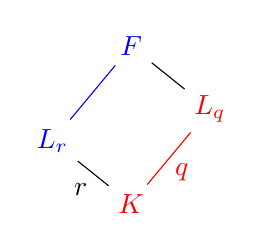
\begin{tikzpicture}

            \node [red] (Q1) at (0,0) {$K$};
            \node [red] (Q2) at (1,1.2) {$L_q$};
            \node [blue] (Q3) at (0,2) {$F$};
            \node [blue] (Q4) at (-1,0.8) {$L_r$};
        
            \draw [red] (Q1)--(Q2) node [pos=0.8, below,inner sep=0.25cm] {$q$};
            \draw (Q1)--(Q4) node [pos=0.9, below,inner sep=0.25cm] {$r$};
            \draw [blue] (Q3)--(Q4);
            \draw (Q2)--(Q3);
        
        \end{tikzpicture}
        \caption[short]{Subfields of a $C_{pq}$-extension}
    \end{figure}

    Again, the result follows immediately from the table and \eqref{eqn_local_contr}.
    
\end{proof}

We are finally ready to prove the main result of this section, from which Theorem \ref{thm_consistent_cyclic} will follow. 

\begin{lemma}\label{lem_Cd_odd}
    Let $d$ be a composite, odd squarefree integer and let $F/K$ be a Galois extension of number fields such that $\Gal(F/K)=C_{d}$. Let $E/\QQ$ be an elliptic curve with semistable reduction at $2$ and $3$ and let $L_k$ be the intermediate fields such that $\Gal(F/L_k)=C_{d/k}$. If 
    $$\Theta_d=\sum_{k\mid d}\mu(k)C_k\in B(C_d),$$
    then $C(\Theta_d)\in\QQss$.
\end{lemma}

\begin{proof}
    Let $n$ be the number of distinct prime numbers dividing $d$, so that $d=p_1\ldots p_n$ for some distinct odd primes $p_i$. We prove this result by induction. The base case for $n=2$ is the content of Lemma \ref{lem_Cpq}. Assume that the result holds for squarefree cyclic Galois extensions with $n-1$ prime factors and consider the two sets of subgroups
    $$\mathcal{A}=\{C_k:p_n\mid k\}\quad\text{and}\quad\mathcal{B}=\{C_k:p_n\nmid k\},$$
    which are clearly a partition of subgroups of $C_d$. Furthermore, the fields $\{F^{C_k}:C_k\in\mathcal{A}\}$ are precisely the intermediate fields of $L_{d/p_n}/K$, while the fields $\{F^{C_k}:C_k\in\mathcal{B}\}$ are the intermediate fields of $F/L_{p_n}$.
    Let 
    $$\Theta_\mathcal{A}=\sum_{H\in\mathcal{A}}\mu(|H|/p_n)H\quad\text{and}\quad\Theta_\mathcal{B}=\sum_{H\in\mathcal{B}}\mu(|H|)H$$
    and we note that
    \begin{equation}\label{eqn_theta}
        \Theta_d=\sum_{k\mid d}\mu(k)C_k=\sum_{p_n\nmid k\mid d}\mu(|C_k|)C_k-\sum_{p_n\mid k\mid d}\mu(|C_k|/p_n)C_k=\Theta_\mathcal{B}-\Theta_\mathcal{A}.
    \end{equation}
    Since $\Gal(L_{d/p_n}/K)=\Gal(F/L_{p_n})=C_{d/p_n}$, it follows from the inductive hypothesis applied to $L_{d/p_n}/K$ and $F/L_{p_n}$ that $C(\Theta_\mathcal{A}),C(\Theta_\mathcal{B})\in\QQss$, and therefore
    $$C(\Theta_d)=\frac{C(\Theta_\mathcal{B})}{C(\Theta_\mathcal{A})}\in\QQss,$$ 
    as desired.
    \begin{figure}[!ht]
        \centering
        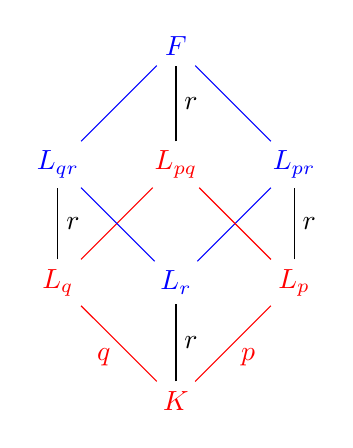
\begin{tikzpicture}

            \node [red] (Q1) at (0,0) {$K$};
            \node [red] (Q2) at (-1.5,1.5) {$L_q$};
            \node [blue] (Q3) at (0,1.5) {$L_r$};
            \node [red] (Q4) at (1.5,1.5) {$L_p$};
            \node [blue] (Q5) at (-1.5,3) {$L_{qr}$};
            \node [red] (Q6) at (0,3) {$L_{pq}$};
            \node [blue] (Q7) at (1.5,3) {$L_{pr}$};
            \node [blue] (Q8) at (0,4.5) {$F$};

            \draw [red] (Q1)--(Q2) node [pos=0.7, below,inner sep=0.25cm] {$q$};
            \draw [red] (Q1)--(Q4) node [pos=0.7, below,inner sep=0.25cm] {$p$};
            \draw (Q1)--(Q3) node [pos=0.5, right,inner sep=0.1cm] {$r$};
            \draw (Q2)--(Q5) node [pos=0.5, right,inner sep=0.1cm] {$r$};
            \draw (Q2)--(Q6) [red];
            \draw (Q3)--(Q5) [blue];
            \draw (Q3)--(Q7) [blue];
            \draw (Q4)--(Q6) [red];
            \draw (Q4)--(Q7) node [pos=0.5, right,inner sep=0.1cm] {$r$};
            \draw (Q5)--(Q8) [blue];
            \draw (Q6)--(Q8) node [pos=0.5, right,inner sep=0.1cm] {$r$};
            \draw (Q7)--(Q8) [blue];
        
        \end{tikzpicture}
        \caption[short]{Partition of $n=3$ into $n=2$. Red fields are in $\mathcal{A}$ while blue fields are in $\mathcal{B}$.}
    \end{figure}
\end{proof}

The proof of Theorem \ref{thm_consistent_cyclic} for odd $d$ is now straightforward.

\begin{proof}[Proof of Theorem \ref{thm_consistent_cyclic} for odd $d$]
    The proof is divided into two cases depending on whether $d$ is the power of a prime or not. Suppose first that $d$ is not, so that $\rad(d)$ is a squarefree \textbf{composite} number. Then $\Theta_d=\sum_{k\mid d}\mu(k)C_k\in B(C_d)$ is the $\psi_d$-relation of a faithful character of $C_d$. The subgroups appearing on $\Theta_d$ are the subgroups of $C_{\rad(d)}$ and therefore by Lemma \ref{lem_Cd_odd} applied to the $C_{\rad(d)}$ extension $F/F^{C_{\rad(d)}}$, it follows that 
    $$C(\Theta_d)\in\QQss,$$ and therefore it is the norm of an element for any quadratic extension of $\QQ$. 

    If $d=q^n$ for some odd prime $q$ and $n\geq1$, then Lemma \ref{lem_relation} shows that $\Theta_d=C_1-C_q$ is the $\psi_d$-relation of a faithful character of $C_d$. Lemma \ref{lem_Cp} applied to the $C_q$ extension $F/F^{C_q}$ proves that 
    $$C(\Theta_d)=\frac{C(C_1)}{C(C_q)}\in N_{\QQ(\sqrt{q^*})/\QQ}(\QQ(\sqrt{q^*})^{\times}).$$ 
    By Lemma \ref{lem_subfields} this is the only quadratic subfield of $\QQ(\zeta_{q^n})$, so the result follows.
\end{proof}

 
\subsubsection{Even Cyclic Extensions}
More care is required to prove Theorem \ref{thm_consistent_cyclic} for even $d$. This difficulty mainly lies in the case when $d$ is only divisible by one odd prime $q$. Consequently, we break down the proof into three distinct cases according to the number of odd prime divisors of $d$. If $d$ has more than one odd prime divisor, then the result follows without much work from Lemma \ref{lem_Cd_odd}, so we prove this first.

\begin{proof}[Proof of Theorem \ref{thm_consistent_cyclic} for even $d$ with more than one odd prime divisor]
    By Remark \ref{rem_radical}, recall that the subgroups present in $\Theta_d$ are precisely those such that $C_k\leq C_{\rad(d)}$, and so following a similar idea to Lemma \ref{lem_Cd_odd}, we define
    $$\mathcal{A}=\{C_k :2\mid k\mid\rad(d)\}\quad\text{and}\quad\mathcal{B}=\{C_k:2\nmid k\mid\rad(d)\},$$
    together with
    $$\Theta_\mathcal{A}=\sum_{H\in\mathcal{A}}\mu(|H|/2)H\quad\text{and}\quad\Theta_\mathcal{B}=\sum_{H\in\mathcal{B}}\mu(|H|)H. $$ 
    For each $k\mid d$, let $L_k=F^{C_{d/k}}$ be the unique subfield of degree $k$ over $K$. The fields $\{F^{C_k}:C_k\in\mathcal{A}\}$ are the intermediate fields of $L_{d/2}/L_{d/\rad(d)}$ and the fields $\{F^{C_k}:C_k\in\mathcal{A}\}$ are the intermediate fields of $F/L_{2d/\rad(d)}$. However, note that 
    $$\Gal(L_{d/2}/L_{d/\rad(d)})=\Gal(F/L_{2d/\rad(d)})=C_{\rad(d)/2},$$
    and by assumption $\rad(d)/2$ is an odd number with more than one prime factor. Then Lemma \ref{lem_subfields} applied to $L_{d/2}/L_{d/\rad(d)}$ and $F/L_{2d/\rad(d)}$ gives $\Theta_\mathcal{A},\Theta_\mathcal{B}\in\QQss$. The calculation in \eqref{eqn_theta} shows that $\Theta_d=\Theta_\mathcal{B}-\Theta_\mathcal{A}$ and therefore 
    $$C(\Theta_d)=\frac{C(\Theta_\mathcal{B})}{C(\Theta_\mathcal{A})}\in\QQss$$
    is the norm of any quadratic extension.
\end{proof}

If $d$ has no odd primes factors, then $d=2^l$ for some $l\geq1$. In that case, we assume in Theorem \ref{thm_consistent_cyclic} that $E$ is semistable, and the proof under this assumption is short. 

\begin{proof}[Proof of Theorem \ref{thm_consistent_cyclic} for $d=2^l$ and semistable $E$]

    If $l=1$, then $\QQ(\zeta_2)=\QQ$, and there is nothing to prove, so assume that $l\geq2$. If $\Gal(F/\QQ)=C_{2^l}$, then 
    $$C(\Theta_d)=\frac{C(C_1)}{C(C_2)}=\frac{C_{E/F}}{C_{E/L_{2^{l-1}}}},$$
    and $F/L_{2^{l-1}}$ is a $C_2$ extension. Importantly, we note that Table \ref{table_Cp} also applies for $q=2$, and therefore $\Cp(\Theta_d)$ is a rational square up to factors of $2$ for any prime $\pp$ of $L_{2^{l-1}}$. Lemma \ref{lem_subfields} shows that the only subfields of $\QQ(\zeta_{2^l})$ are $\QQ(i),\QQ(\sqrt{2})$ and $\QQ(\sqrt{-2})$, and since
    $$2=\Norm_{\QQ(i)}(1+i)=\Norm_{\QQ(\sqrt{-2})}(2)=\Norm_{\QQ(\sqrt{2})}(2+\sqrt{2}),$$
    it follows that $\Cp(\Theta_d)$ is a norm from every quadratic subfield of $\QQ(\zeta_{2^l})$, and the result follows.
\end{proof}

The remaining of this section is therefore devoted to the case when $d$ is divisible by one odd prime $q$, so $d=2^mq^n$. 
%When $d$ has this form, then $\Theta_d=C_1-C_2-C_q+C_{2q}$ and therefore fix $\Theta_d$ to have this expression for the remaining of this section. 
Recall that the quadratic subfields of $\QQ(\zeta_{2^mq^n})$ depend on whether $m=1$, $m=2$ or $m\geq 3$. Consequently, we prove three results that will be essential to prove the general version of each different case. The first covers the case $m=1$.

\begin{lemma}\label{lem_C2p}
    Let $q$ be an odd prime and let $F/K$ be a Galois extension of number fields such that $\Gal(F/K)=C_{2q}$ and let $L_k=F^{C_{2q/k}}$ be the intermediate fields such that $[L_k:K]=k$. Let $E/\QQ$ be an elliptic curve and let $\Theta_{2q}=C_{2q}-C_q-C_2+C_1\in B(C_{2q})$. Then
    $$C(\Theta_{2q})=\frac{C_{E/F}C_{E/K}}{C_{E/L_2}C_{E/L_q}}$$
    is a norm from $\QQ(\sqrt{q^*})$.
\end{lemma}

\begin{proof}
    Similarly to the proofs of Lemma \ref{lem_Cp} and \ref{lem_Cpq}, let $\pp$ be a prime in $K$ and assume that $\Delta_E=\Delta_{E,\pp}^{\min}$. The splitting behaviour of a prime $\pp$ in $K$ is again determined by $e_\pp$ and $f_\pp$ and therefore if $\pp$ has multiplicative reduction $\Dp(\Theta_{2q})=1$ and the following table records $\Tp(\Theta_{2q})$.

    \begin{table}[!ht]
        \centering
        \begin{tabular}{|l|l|l|l|l|l|l|}
        \hline
        $e_\pp$ & $f_\pp$  & $\Tp(C_{2q})$ & $\Tp(C_2)$ & $\Tp(C_q)$ & $\Tp(C_1)$ & $\Tp(\Theta_{2q})$ \\ \hline
        $1$ & $1$ & $n;\tilde{n}$ & $n^q;\tilde{n}^q$ & $n^2;\tilde{n}^2$ & $n^{2q};\tilde{n}^{2q}$ & $\square$ \\ \hline
        $1$ & $q$ & $n;\tilde{n}$ & $n;\tilde{n}$ & $n^2;\tilde{n}^2$ & $n^2;\tilde{n}^2$ & $\square$ \\ \hline
        $1$ & $2$ & $n;\tilde{n}$ & $n^q;\tilde{n}^q$ & $n;n$ & $n^q;n^q$ & $\square$ \\ \hline
        $1$ & $2q$ & $n;\tilde{n}$ & $n;\tilde{n}$ & $n;n$ & $n;n$ & $\square$ \\ \hline
        $q$ & $1$ & $n;\tilde{n}$ & $qn;\tilde{n}$ & $n^2;\tilde{n}^2$ & $q^2n^2;\tilde{n}^2$ & $q\square;\square$ \\ \hline
        $q$ & $2$ & $n;\tilde{n}$ & $qn;\tilde{n}$ & $n;n$ & $qn;n$ & $\square$ \\ \hline
        $2$ & $1$ & $n;\tilde{n}$ & $n^q;\tilde{n}^q$ & $2n;1$ & $2^qn^q;1^q$ & $\square$ \\ \hline
        $2$ & $q$ & $n;\tilde{n}$ & $n;\tilde{n}$ & $2n;1$ & $2n;1$ & $\square$ \\ \hline
        $2q$ & $1$ & $n;\tilde{n}$ & $qn;\tilde{n}$ & $2n;1$ & $2qn;1$ & $\square$ \\ \hline
        \end{tabular}
        \caption{Contribution of multiplicative reduction primes in a $C_{2q}$ extension.}
    \end{table}

    Since $q$ is a norm from $\QQ(\sqrt{q^*})$, then $\Tp(\Theta_{2q})$ is also a norm. Now assume that $\pp$ has additive reduction and let $p\ZZ=\pp\cap\QQ$. We first consider the contribution of the Tamagawa numbers. Note that $L_q/K$ and $F/L_2$ are $C_q$ extensions and therefore $\Tp(\Theta_{2q})\in\QQss$ if $q\neq 3$ and a square up to factors of $3$ if $q=3$. In either case, $\Tp(\Theta_{2q})$ is a norm from $\QQ(\sqrt{q^*})$.

    Finally, to compute $\Dp(\Theta_{2q})$, let $n=\nu_\pp(\Delta_{E,\pp}^{\min})$ and note that all terms cancel unless $\pp$ ramifies in $F$. If $e_\pp=2$, then
    \begin{equation}\label{eqn_ep=2}
        \Dp(C_{2q})=\Dp(C_2)=1,\quad \Dp(C_q)=N(\pp)^{\floor{\frac{2n}{12}}}\quad\text{and}\quad \Dp(C_1)=N(\pp)^{q\floor{\frac{2n}{12}}},
    \end{equation}
    and therefore $D(\Theta_{2q})=N(\pp)^{(q-1)\floor{n/6}}\in\QQss$, a rational square. If $q\mid e_\pp$, then $q\mid N(\pp)-1$ by Proposition \ref{prop_totally_ramified}, and the reasoning is now identical to Lemma \ref{lem_Cp}. Write $N(\pp)=p^s$ for some $s\geq1$ and note that $\Dp(\Theta_{2q})\in\QQss$ if $s$ is even. Hence, we assume that $s$ is odd. In this case, $p=q$ if $(L_q)_\fP/K_\pp$ is wildly ramified and $p$ splits in $\QQ(q^*)$ if $(L_q)_\fP/K_\pp$ is tamely ramified. In either case, by Corollaries \ref{p-norm} and \ref{cor_psplit_pnorm}, $p$ is a norm from $\QQ(\sqrt{q^*})$, and hence so is $\Dp(\Theta_{2q})$.
    The result follows again from \eqref{eqn_local_contr}.
\end{proof}

Following this, we state and prove the analogous result for $m=2$.

\begin{lemma}\label{lem_C4p}
    Let $q$ be an odd prime and let $F/K$ be a Galois extension of number fields such that $\Gal(F/K)=C_{4q}$ and let $L_k=F^{C_{4q/k}}$ be the intermediate fields such that $[L_k:K]=k$. Let $E/\QQ$ be an elliptic curve with semistable reduction at $2$ and $3$ and let $\Theta_{4q}=C_1-C_2-C_q+C_{2q}$. Then 
    $$C(\Theta_{4q})=\frac{C_{E/F}C_{E/L_2}}{C_{E/L_4}C_{E/L_{2q}}}$$
    is a norm from $\QQ(i),\QQ(\sqrt{q})$ and $\QQ(\sqrt{-q})$. Moreover, $\Tp(\Theta_{4q})\in\QQss$ for any prime $\pp$ in $K$, and $\Dp(\Theta_{4q})\in\QQss$ unless $E$ has additive reduction at $\pp$ and $\pp$ is totally ramified in $F/K$.
\end{lemma}

\begin{proof}
    All fields appearing in the product are intermediate fields of $F/L_2$, and $\Gal(F/L_2)=C_{2q}$. Let $\pp$ be a prime in $K$, let $\bar\pp\mid\pp$ be a prime above $\pp$ in $L_2$ and let $p\ZZ=\pp\cap\QQ$. Assume also that $\Delta_E=\Delta_{E,\pp}^{\min}$. Lemma \ref{lem_C2p} shows that if $E$ has multiplicative reduction over $\bar\pp$, $C_{\fP\mid\bar\pp}(\Theta_{4q})\in\QQss$ unless $e_{\bar\pp}=q$ and $f_{\bar\pp}=1$ over $F$. When this holds, $\bar\pp$ ramifies in $L_{2q}/L_2$ and is split in $L_4/L_2$, and this forces $\pp$ to split in $L_2/K$ too. Hence, $\pp=\bar\pp\bar\pp'$ for two \textbf{distinct} primes in $K$ that have the same local behaviour and therefore $\Cp(\Theta_{4q})=C_{\fP\mid\bar\pp}(\Theta_{4q})C_{\fP\mid\bar\pp'}(\Theta_{4q})=C_{\fP\mid\bar\pp}(\Theta_{4q})^2\in\QQss$, as desired.

    \begin{figure}[!ht]
        \centering
        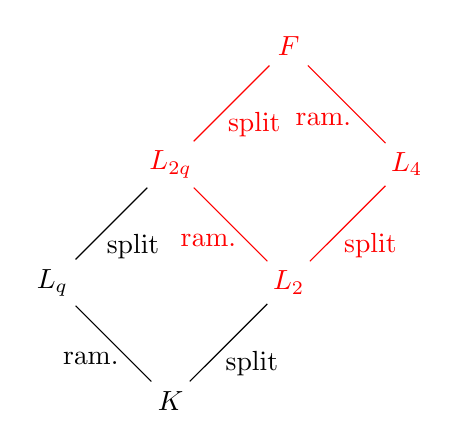
\begin{tikzpicture}

            \node (Q1) at (0,0) {$K$};
            \node (Q2) at (-1.5,1.5) {$L_q$};
            \node [red] (Q3) at (3,3) {$L_4$};
            \node [red] (Q4) at (1.5,1.5) {$L_2$};
            \node [red] (Q5) at (1.5,4.5) {$F$};
            \node [red] (Q6) at (0,3) {$L_{2q}$};
            

            \draw (Q1)--(Q2) node [pos=0.8, below,inner sep=0.4cm] {ram.};
            \draw (Q1)--(Q4) node [pos=0.8, below,inner sep=0.4cm] {split};
            \draw (Q2)--(Q6) node [pos=0.8, below,inner sep=0.4cm] {split};
            \draw [red] (Q3)--(Q5) node [pos=0.8, below,inner sep=0.4cm] {ram.};
            \draw [red] (Q4)--(Q6) node [pos=0.8, below,inner sep=0.4cm] {ram.};
            \draw [red] (Q6)--(Q5) node [pos=0.8, below,inner sep=0.4cm] {split};
            \draw [red] (Q4)--(Q3) node [pos=0.8, below,inner sep=0.4cm] {split};
        \end{tikzpicture}
        \caption[short]{\centering Field diagram for a $C_{4q}$ extension, together with the splitting\newline behaviour of a prime $\pp$ in $L_2$ with $e_\pp=q$ and $f_\pp=1$ over $F$.}
    \end{figure}

    Assume now that $E$ has additive reduction over $\bar\pp$. When $q=3$, controlling the Tamagawa numbers is lengthy, so we leave it for the end. We calculate first $\Dp(\Theta_{4q})$, which is $1$ unless $\bar\pp$ ramifies in $L/F_2$ (equivalently, $\pp$ ramifies in $L/K$). If $\pp$ is inert in $L_2/K$, then $N(\bar{\pp})\in\QQss$ and hence the size of all residues fields above $\pp$ are also squares and consequently $\Dp(\Theta_{4q})\in\QQss$ using Lemma \ref{lem_Dterms}. If $\pp=\bar\pp\bar\pp'$ splits, then $D_{\fP\mid\bar\fp}(\Theta_{4q})=D_{\fP\mid\bar\fp'}(\Theta_{4q})$, and therefore $\Dp(\Theta_{4_q})\in\QQss$ too. Finally, assume that $\pp=\bar\pp^2$ ramifies in $L_2/K$, which implies that $\bar\fp$ also ramifies in $L_4/L_2$. On the other hand, if $\bar\pp$ is unramified at $L_{2q}/L_2$, \eqref{eqn_ep=2} during the proof of Lemma \ref{lem_C2p} shows that $\Dp(\Theta_{4q})\in\QQss$ too. 

    We are therefore left with the case where $\pp$ is totally ramified in $F/K$, and Proposition \ref{prop_totally_ramified} implies that $4q\mid N(\pp)-1$. If we let $n=\nu_{\pp}(\Delta_{E,\pp}^{\min})$, Lemma \ref{lem_Dterms} implies that 
    \begin{equation*}\label{eqn_DtermsC4p}
        \Dp(\Theta_{4q})=N(\pp)^{\floor{\frac{n}{6}}-\floor{\frac{n}{3}}-\floor{\frac{qn}{6}}+\floor{\frac{qn}{3}}}.
    \end{equation*}
    Again, the parity of the expression only depends on $q,n\pmod{12}$. One can easily check that for $n\in\{2,3,4,6,8,9,10\}$ and $q\in\{1,5,7,11\}$, the above expression is a square unless $q\equiv 3\pmod{4}$ and $n$ is odd, so we assume this is the case. Write $N(\pp)=p^s$ for some $s\geq1$, which satisfies $p^s\equiv1\pmod{4q}$. If $s$ is even, then $\Dp(\Theta_{4q})\in\QQss$, so assume that $s$ is odd. Since $p^s\equiv1\pmod{4}$, this implies that $p\equiv1\pmod{4}$ and hence $p$ is a norm from $\QQ(i)$, which implies that $\Dp(\Theta_{4q})$ is a norm from $\QQ(i)$ too. Furthermore, the fact that $p^s\equiv1\pmod{4q}$ implies that
    $$\left(\frac{-q}{p}\right)=\left(\frac{q}{p}\right)=\left(\frac{p}{q}\right)=\left(\frac{p^s}{q}\right)=1,$$
    and therefore $p$ splits both in $\QQ(\sqrt{q})$ and $\QQ(\sqrt{-q})$. Since $q\equiv3\pmod{4}$, both fields have odd class number (Theorem \ref{thm_class_number}), and hence $p$ and $\Dp(\Theta_{4q})$ are norms from $\QQ(\sqrt{q})$ and $\QQ(\sqrt{-q})$ as desired. 

    Finally, we discuss Tamagawa numbers. Note that $L_{2q}/L_2$ and $F/L_4$ are $C_q$ extensions and therefore by Lemma \ref{lem_Cp} it follows that $\Dp(\Theta_{4q})\in\QQss$ if $q\neq3$. If $q=3$, it is also the case that $\Dp(\Theta_{4q})\in\QQss$, but more work is required. We prove this as a separate lemma, from which the result follows.    
\end{proof}

\begin{lemma}
    Let $L/K$ be a Galois extension of number fields with $\Gal(L/K)=C_{12}$ and let $L_k=F^{C_{12/k}}$ be the intermediate fields such that $[L_k:K]=k$. Let $E/\QQ$ be an elliptic curve and let $\pp$ be a prime in $K$ not dividing $2$ or $3$ such that $E$ has potentially good reduction at $\pp$. If $\Theta_{12}=C_1-C_2-C_3+C_6\in B(C_{12})$, then $$\Tp(\Theta_{12})=\frac{\Tp(E/F)\Tp(E/L_2)}{\Tp(E/L_6)\Tp(E/L_4)}\in\QQss.$$
\end{lemma}
\begin{proof}
    Let $\bar\pp$ be a prime in $L_2$ above $\pp$ and let $n=\nu_{\bar\pp}(\Delta_{E,\bar\pp}^{\min})$ be the minimal discriminant of $E$ at $\bar\pp$. If $\pp$ is unramified in $L_3/K$, then so is $\bar\pp$ in $L_6/L_2$ and the primes above them in $F/L_4$. From Lemma \ref{lem_Cp}, we know that that the product of Tamagawa numbers in unramified $C_3$ extensions is a square, so assume that $\pp$ ramifies in $L_3/K$.

    The proof is now divided in three cases, depending on the splitting behaviour of $\pp$ in $L_2$. If $\pp$ splits in $L_2/K$, then $\pp=\bar\pp\bar\pp'$ where $\bar\pp$ and $\bar\pp'$ have the same local behaviour. Therefore, $T_{\fP\mid\pp}(\Theta_{12})=T_{\fP\mid\bar\pp}(\Theta_{12})T_{\fP\mid\bar\pp'}(\Theta_{12})\in\QQss$. 
    
    Next, suppose that $\pp$ is inert in $L_2/K$, which implies that $\bar\pp$ is either inert or ramified in $L_4/L_2$. Let $\fP$ be the prime in $L_4$ above $\bar\pp$. If $\bar\pp$ is inert in $L_4/L_2$, then the valuation of the minimal discriminant of $E$ at $\fP$ is also $n$ and the splitting behaviour of $\bar\pp$ in $L_6/L_2$ coincides with the splitting behaviour of $\fP$ in $F/L_4$. Hence, 
    $$\frac{\Tp(E/F)}{\Tp(E/L_4)}=\frac{\Tp(E/L_6)}{\Tp(E/L_2)},$$
    and therefore $\Tp(\Theta_{12})=1$. The case where $\bar\pp$ is ramified in $L_4/L_2$ is more subtle. We have already seen that in ramified $C_3$ extensions we cannot obtain factors of $2$. Upon inspection of Lemma \ref{lem_add_tam}, one can easily show that the Tamagawa numbers cancel out if $\gcd(n,12)\in\{3,4,6,12\}$, so we only need to consider the case $\gcd(n,12)=2$. Since $\Gal((L_4)_\fP/K_\pp)=C_4$ and $e_{\fP\mid\pp}=f_{\fP\mid\pp}=2$, Lemma \ref{lem_notthree} shows that $\sqrt{B}\not\in F_{\fP}$ and therefore $c_\fP(E/F)=1$, which imples that $\Dp(\Theta_{12})\in\QQss$.

    Finally, assume that $\pp$ ramifies in $L_2/K$ so that $\pp=\bar\pp^2$. This immediately implies that $\bar\pp$ also ramifies in $L_4/L_2$, and therefore $\pp$ is totally ramified in $F/K$. As mentioned above, the Tamagawa numbers cancel unless $\gcd(n,12)=2$. However, recall that $E$ has potentially good reduction at $\pp$, and since $\pp=\bar\pp^2$ ramifies, then the valuation of the minimal discriminant at $\pp$ is $n/2$ or $(n+12)/2$. But then $\gcd(\nu_\pp(\Delta_{E,\pp}^{\min}),12)=\gcd(n/2,12)=1$, a contradiction. Hence, $\Tp(\Theta_{12})\in\QQss$ as desired.
\end{proof}

Finally, we state and prove the last result, from which the case $m\geq3$ follows easily. One needs to check that the product of local factors is the norm of many quadratic subfields; thankfully, Lemma \ref{lem_C4p} has done most of work required.

\begin{lemma}\label{lem_C8p}
    Let $q$ be an odd prime and let $F/K$ be a Galois extension of number fields such that $\Gal(F/K)=C_{8q}$ and let $L_k=F^{C_{8q/k}}$ be the intermediate fields such that $[L_k:K]=k$. Let $E/\QQ$ be an elliptic curve with semistable reduction at $2$ and $3$ and let $\Theta_{8q}=C_1-C_2-C_q+C_{2q}$. Then 
    $$C(\Theta_{8q})=\frac{C_{E/F}C_{E/L_4}}{C_{E/L_8}C_{E/L_{4q}}}\in\QQss.$$
    %is a norm from $\QQ(\sqrt{D})$ for each $D\in\{-1,\pm2,\pm q,\pm 2q\}$.
\end{lemma}

\begin{proof}
    We prove the result locally for all primes in $L_2$, and note $\Gal(F/L_2)=4q$. Let $\bar\pp$ and assume that $\Delta_E=\Delta_{E,\bar\pp}^{\min}$. Since the relation $\Theta_{4q}=C_1-C_2-C_q+C_{2q}\in B(C_{4q})$ has the same fixed fields as $\Theta_{8q}$, by Lemma \ref{lem_C4p}, we know that $\Tpb(\Theta_{8q})\in\QQss$ for any $\bar\pp$ and $\Dpb(\Theta_{8q})\in\QQss$ too unless $\bar\pp$ is totally ramified in $F/L_2$ and $E$ has potentially good reduction at $\bar\pp$, so assume this is the case. If $\pp=\bar\pp\cap K$, then it also follows that $\pp$ is totally ramified in $F/K$ and $E$ has potentially good reduction at $\pp$. If $n=\nu_{\bar\pp}(\Delta_{E,\bar\pp}^{\min})$, then recall from Lemma \ref{lem_C4p} that 
    $$\Dpb(\Theta_{8q})=N(\bar\pp)^{\floor{\frac{n}{6}}-\floor{\frac{n}{3}}-\floor{\frac{qn}{6}}+\floor{\frac{qn}{3}}},$$
    and that the exponent is even unless $n$ is odd and $q\equiv 3\pmod{4}$. However, $\pp=\bar\pp^2$ is ramified in $L_2/K$ and therefore $n\equiv 2\nu_\pp(\Delta_{E,\pp}^{\min})\pmod{12}$. That is, $n$ is even and therefore $\Dpb(\Theta_{8q})\in\QQss$ as desired.
\end{proof}
%%% THIS IS ALL PROBABLY NOT NEEDED NOW
%Again, $\Dp(\Theta_{8q})$ does not change up to squares if $\Delta_{E}$ is reescaled so assume that $\Delta_{E}=\Delta_{E,\pp}^{\min}$. Under these assumptions, $\Dpb(\Theta_{8q})=\Dp(\Theta_{8q})$ is a power of $N(\pp)=N(\bar\pp)=p^s$ for some rational prime $p$ and $s\geq1$. If $s$ is even, then $\Dpb(\Theta_{8q})\in\QQss$, so assume that $s$ is odd. In addition, by Proposition \ref{prop_totally_ramified}, it follows that $p^s\equiv 1\pmod{8q}$. Since $s$ is odd and $(\ZZ/8\ZZ)^*=C_2\times C_2$, it follows that $p\equiv 1\pmod{8}$ and therefore
%\begin{equation}\label{eqn_psplitsin2}
%    \left(\frac{-1}{p}\right)=\left(\frac{2}{p}\right)=\left(\frac{-2}{p}\right)=1.
%\end{equation}
%Furthermore, since $p^s\equiv1\pmod{8s}$ and $s$ is odd, then 
%\begin{equation}\label{eqn_psplitsinq}
%    \left(\frac{-q}{p}\right)=\left(\frac{q}{p}\right)=\left(\frac{p}{q}\right)=1.
%\end{equation}
%Combining \eqref{eqn_psplitsin2} and \eqref{eqn_psplitsinq} together with multiplicativity of the Legendre symbol, it follows that $p$ splits in every quadratic subfield $\QQ(\sqrt{D})$ for $D\in\{-1,\pm2,\pm q,\pm2q\}$.


We are now ready to prove the remaining case of Theorem \ref{thm_consistent_cyclic}.

\begin{proof}[Proof of Theorem \ref{thm_consistent_cyclic} for $d$ even and with one odd prime factor.]
    In this case, write $d=2^mq^n$ for $n,m\geq 1$ and note that $\Theta_{d}=C_1-C_2-C_q+C_{2q}$ is the $\psi_d$-relation of a faithful character of $C_d$. If $m=1$, Lemma \ref{lem_C2p} applied to the $C_{2q}$ extension $F/F^{C_{2q}}$ shows that $C(\Theta_d)$ is a norm from $\QQ(\sqrt{q^*})$, which is the only subfield of $\QQ(\zeta_{2q^n})$ by Lemma \ref{lem_subfields}. If $m=2$, then Lemma \ref{lem_C4p} applied to the $C_{4q}$ extension $F/F^{C_{4q}}$ shows that $C(\Theta_{d})$ is a norm from $\QQ(i),\QQ(\sqrt{q})$ and $\QQ(\sqrt{-q})$, which are all quadratic subfields of $\QQ(\zeta_{4q^n})$. Finally, if $m\geq3$, Lemma \ref{lem_C8p} applied to $F/F^{C_{8q}}$ shows that $C(\Theta_{8q})\in\QQss$, which is the norm from any quadratic subfield. The result follows.
\end{proof}



\subsection{Norm Relations in Odd Order Extensions}\label{subsec-odd}

We now prove a result analogous to the previous section, but when $F / \bQ$ is any Galois extension of odd order. %The reason one would expect that our norm relations test never forces rank growth in this case is because root number computations do not, as we now show.

%\begin{lemma}
% Let $F / \bQ$ be an odd Galois extension with $G = \Gal(F / \bQ)$. Then $w(E / \bQ) = w(E / F^H)$ for all $H \leq G$. 
%\end{lemma}

%\begin{proof}
%Consider $H \leq G$ and intermediate field $F^H$. Then $\Ind_H^G \trivial \simeq \trivial \oplus \rho \oplus \rho^*$ for some non self-dual representation $\rho$ of $G$, since the only self-dual representation of an odd-order group is the trivial representation. Therefore by Proposition \ref{compute-root-twist}, $w(E / F^H) = w(E / F)w(E, \rho \oplus \rho^*)$ and $w(E, \rho \oplus \rho^*) = 1$. Hence $w(E / \bQ) = w(E / F^H)$ for all $H \leq G$. 
%\end{proof}

%Therefore once we assume that $\rk E / \bQ = 0$, the parity conjecture tells us that $\rk E / F^H$ is even for all $H \leq G$, which does not force it to be non-zero. 


\begin{thm}\label{odd-exts}
 Let $E / \bQ$ be an elliptic curve, $F / \bQ$ be an extension of odd order with Galois group $G$. 
 
Assume that $E$ has good or multiplicative reduction at $2$ and $3$. 
Take any representation $\rho$ of $G$ with quadratic subfield $\bQ(\sqrt{D}) \subset \bQ(\rho)$ and relation
\begin{equation*}\label{odd-exp} \repnorm{\rho}^{\oplus m} =
 \left(\bigoplus_{\mathfrak{g}\in\Gal(\QQ(\rho)/\QQ)}\rho^{\mathfrak{g}}\right)^{\oplus m }=\bigoplus_i\Ind_{F_i/\QQ}\mathds{1}\ominus\bigoplus_j\Ind_{F'_j/\QQ}\mathds{1}
\end{equation*}
 as in Theorem \ref{thm_positive_rank}. Then
 \[ \frac{\prod_i C_{E/F_i}}{\prod_j C_{E/F_j'}}  \in 
    \begin{cases}
        N_{\bQ(\sqrt{D}) / \bQ}(\bQ(\sqrt{D})^{\times}) & m \ \text{odd}, \\
        (\bQ^{\times})^2 & m \ \text{even}.
    \end{cases} \] 
    In other words, one cannot use Theorem \ref{thm_positive_rank} to conclude that $E / F$ must have positive rank. 
\end{thm}

As in Remark \ref{rephrase-thm}, replacing $\rho$ by the sum of its conjugates by elements of $ \Gal(\bQ(\rho) / \bQ(\sqrt{D}))$, we may assume that $\bQ(\rho) = \bQ(\sqrt{D})$. We take $D \in \bZ \backslash \{0,1 \}$ to be squarefree.

The product of terms we are computing is $C(\Theta)$, where $C \colon \B(G) \to \bQ^{\times}$ is given by $C \colon H \mapsto C_{E / F^H}$, and $\Theta$ is any $\rho$-relation.
We break up the function $C$ into $C = \prod_p C_{\fP \mid p} = \prod_p T_{\fP \mid p} \cdot D_{\fP \mid p}$, ranging over primes $p \in \bQ$,
as defined in Notation \ref{not_contr_fns}.
We showed that
\begin{equation*}\label{Dp-loc}
C_{\fP \mid p} = (D_p, C_v)
\end{equation*}
where $C_v$ is a function on $\B(D_p)$ sending $H \mapsto C_v(E / F_w^H)$, for $D_p = \Gal(F_w / \bQ_p)$. The following result will allow us to apply some results from $\S$\ref{sec-norm-rels}.

\begin{thm}\label{odd-c-brauer}
    When $D_p$ has odd order, $C_v(\Psi) \in (\bQ^{\times})^2$ for any Brauer relation $\Psi \in \B(D_p)$. 
\end{thm}

\begin{proof}
    This follows from \cite[Theorem 2.47]{reg-const} and \cite[Theorem 3.2  (Tam)]{reg-const}.
\end{proof}

\begin{cor}
It is enough to prove Theorem \ref{odd-exts} when $m$ is the order of $\repnorm{\rho}$ in $\C(G)$. Thus we need to prove that, given any $
\Theta \in \B(G)$ such that $\bC[\Theta] \simeq \repnorm{\rho}^{\oplus m}$, $\Theta$ is a norm relation for the function $C$. 
\end{cor}

\begin{proof}
    Since $\bQ(\rho)$ is quadratic, we have that rational squares are norms from $\bQ(\rho)$. As $G$ is odd, any choice of $D_p$ is odd. It follows from Theorem \ref{odd-c-brauer} that $C(\Psi) \in (\bQ^{\times})^2$ for all Brauer relations $\Psi \in \B(G)$. Therefore by Proposition \ref{min-to-all}, it is enough to prove Theorem \ref{odd-exts} when $m$ is the order of $\repnorm{\rho}$ in $\C(G)$. Then $m$ divides $|G|$, hence is odd.
\end{proof}

Let $\tau$ be the generator of $\Gal(\bQ(\sqrt{D}) / \bQ)$.
Let $\ff$ be the smallest integer such that $\bQ(\sqrt{D}) \subset \bQ(\zeta_{\ff})$. Then $\ff \mid |G|$, hence is odd. By Remark \ref{conductor}, $\ff = |D|$ and $D \equiv 1 \pmod 4$. The following shows that it is only of interest to consider decomposition groups of exponent divisible by $\ff$.

\begin{cor}\label{rational-res-2}
    Let the exponent of $D_p$ be $b$. If $\ff \nmid b$, then $C_{\fP \mid p}(\Theta) \in (\bQ^{\times})^2$.
\end{cor}

\begin{proof}
    One has $\bQ(\rho) \subset \bQ(\zeta_b) \implies \ff \mid b$ by minimality of $\ff$. Since $\ff \nmid b$, we have $\bQ(\rho) \not\subset \bQ(\zeta_b)$, so $\bQ(\Res_{D_p} \rho) = \bQ$. The corollary then follows from Proposition \ref{rational-res} and Theorem \ref{odd-c-brauer}, noting that since $\C(D_p)$ is odd, multiplication by $2$ is injective. 
\end{proof}

Fix $\Theta = \sum_i n_i H_i \in \B(G)$ with $\bC[\Theta] \simeq \repnorm{\rho}^{\oplus m}$. We prove that at each prime $p$, $C_{\fP \mid p}(\Theta)$ is the norm of an element of $\bQ(\rho)$.  As observed, this depends on $D_p$ and $I_p$. As we deal with each local factor individually, we argue that one can take $D_p = I_p$.

\begin{lemma}\label{tam-up-to-square}
    Let $E / K$ be an elliptic curve. Let $K' / K$ be an extension of number fields odd degree, unramified at the place $v$ of $K$. Then $C_w(E / K') \equiv C_v(E / K) \mod (\bQ^{\times})^2$ for any place $w$ of $K'$ with $ w \mid v$. 
\end{lemma}

\begin{proof}
This is automatic for good reduction and split multiplicative reduction. It is also clear for non-split multiplicative reduction since the residue degree cannot be even (so the reduction type remains non-split at $w$). For additive reduction, see \cite[Lemma 3.12]{reg-const}.
\end{proof}

\begin{lemma}\label{DeqI}
    At a prime $p$, we may assume that $D_p = I_p$ when computing $C_{\fP \mid p}(\Theta)$. 
\end{lemma}

\begin{proof}
Let $p$ have residue degree $f_p$. Let $L / \bQ$ be a Galois extension of degree $f_p$ with cyclic Galois group, such that $p$ is inert in $L$. Further ensure that $F \cap L = \bQ$. Then $\Gal(FL / L) = G$. Let $F_i = F^{H_i}$ and $L_i = F_i L$.

Let $v$ be a place over $p$ in $F_i$. The extension $L_i / F_i$ is Galois, so $v$ is either split or inert in $L_i$.
We claim that $C_v(E / F_i) \equiv \prod_{w | v} C_w(E / L_i) \mod (\bQ^{\times})^2$. Indeed, the number of terms in the product on the right is odd, and by Lemma \ref{tam-up-to-square} $C_v(E / F_i) \equiv C_w(E / L_i) \mod (\bQ^{\times})^2$. 
Letting $C_{\fP \mid p}'$ be the function on $\B(G)$ defined as in \eqref{not_contr_fns} but with $\bQ$, $F$ replaced by $L$, $FL$, we see that $C_{\fP \mid p}'(\Theta) \equiv C_{\fP \mid p}(\Theta) \mod (\bQ^{\times})^2$. 
Thus it is equivalent to do our computation in $FL / L$, but here $p$ has residue degree $1$.
\end{proof}

To prove Theorem \ref{odd-exts}, we proceed by computing $C_{\fP \mid p}(\Theta)$ for each reduction type.

\subsubsection*{Good reduction}
If $E / \bQ$ has good reduction at $p$, then by Proposition \ref{prop_local_fns}(i), $C_{\fP \mid p} = 1$.

\subsubsection*{Multiplicative reduction}

\begin{lemma}
Let $E / \bQ_p$ have non-split multiplicative reduction. Then $C_{\fP \mid p}(\Theta) \in (\bQ^{\times})^2$.
\end{lemma}

\begin{proof}
Since $D_p = I_p$, all primes above $p$ have residue degree $1$. Moreover, the ramification degrees are always odd. Thus by Proposition \ref{prop_local_fns}(iii), $C_{\fP \mid p}  = (D_p, \alpha)$
where $\alpha$ is the constant function on $\B(D_p)$ with $\alpha \in \{1, 2\}$, depending on $v_p(\Delta)$ being even or odd. By Proposition \ref{const-fns}, it follows that $C_{\fP \mid p}(\Theta) \in (\bQ^{\times})^2$.
\end{proof}

Now suppose $E / \bQ_p$ has split multiplicative reduction. The reduction type remains split at all places above $p$ within sub-extensions of $F / \bQ$. Let $v_p(\Delta) = n$. Then by Proposition \ref{prop_local_fns}(ii), 
\[ C_{\fP \mid p} = (D_p, D_p, en). \]
Since the $n$ factor is constant, $(D_p, D_p, en)(\Theta) \equiv (D_p, D_p, e)(\Theta) \mod (\bQ^{\times}) ^2$ by Proposition \ref{const-fns} .

We have $D_p = I_p = P_p \ltimes C_l$, where $P_p \triangleleft I_p$ is wild inertia, and $C_l = I_p / P_p$ is the tame quotient. $C_l$ is a cyclic group, with $l \mid p^f - 1 = p - 1$. By Corollary \ref{rational-res-2}, we may consider such $D_p$ with exponent  $p^u l$ for some $u \geq 0$ such that $\ff \mid p^u l$. To compute $C_{\fP \mid p}(\Theta)$, we reduce to the tame quotient.

\begin{lemma}
Let $g \colon \B(C_l) \to \bQ^{\times}$ be defined by $H \mapsto [C_l \colon H] = \dim \bC[C_l / H]$. Let $\Psi = P_p \cdot \Res_{D_p} \Theta / P_p \in \B(C_l)$ Then $(D_p, D_p, e)(\Theta)$ and $g(\Psi)$ differ by a (possible) factor of $p$. 
\end{lemma}

\begin{proof}
%Now, $(D_p, D_p, e)(\Theta)$ is the product of ramification indices at primes above $p$. We separate the $p$-part and tame part of this expression.
Recall that the ramification index of a place $w$ above $p$ corresponding to the double coset $H_i x D_p$ has ramification degree $e_w = \frac{|I_p|}{|H_i \cap I_p^x|} =\frac{|I_p|}{|I_p \cap H^{x^{-1}}|}$.
This is the dimension of the permutation representation $\bC[D_p / D_p \cap H^{x^{-1}}]$.
Let  $D_p \cap H^{x^{-1}} = P' \ltimes C_a$ where $P' \leq P$ and $a | l$. Then the ramification index is $\frac{|P|}{|P'|}\cdot \frac{l}{a}$. 
Taking fixed points under wild inertia, one has the following isomorphism of $D_p$-representations  $$\bC[D_p / D_p \cap H^{x^{-1}}]^{P_p} \simeq \bC[D_p / P_p (D_p \cap H^{x^{-1}})] \simeq \bC[D_p / P_p \ltimes C_a].$$ This permutation representation has dimension $\frac{l}{a}$, so we've killed off the $p$-part. 
Then $$\bC[\Res_{D_p} \Theta]^{P_p} \simeq \left(\Res_{D_p} \rho^{\oplus m} \oplus \tau\left(\Res_{D_p}\rho^{\oplus m}\right)\right)^{P_p},$$
and we can consider these as representations of $D_p / P_p = C_l$.
It follows that $(D_p, D_p, e)(\Theta)$ differs from $g(\Psi)$ up to a (possible) factor of $p$. 
\end{proof}

Now we show that this factor of $p$ is a norm from $\fieldnorm{\rho}$.
Note that if $p = 2$ then $P_p = 1$ since $|P_p| \mid |G|$ which is odd. So we only need to consider this factor of $p$ for $p$ odd.

\begin{lemma}\label{p-norm-odd}
    Let $K = \bQ(\sqrt{D})$, with $\ff$ the smallest positive integer such that $K \subset \bQ(\zeta_{\ff})$. Suppose that $\ff$ is odd. Let $\ff \mid p^u l $, for some odd prime $p$, $u \geq 0$ and $l$ such that $p \equiv 1 \pmod l$. Then $p$ is the norm of an element from $K^{\times}$.
\end{lemma}

\begin{proof}
    Since $\ff$ is odd, one has $D = \prod_{q | \ff} q^*$, the product being taken over primes dividing $\ff$. Note that if $q \not= p$, then since $q \mid l$, we have $p \equiv 1 \pmod l \implies p \equiv 1 \pmod q$. By Corollary \ref{p-one-mod-disc},  $p$ is the norm of a principal fractional ideal of $K$, and by Theorem \ref{p-norm-elem-1} or Theorem \ref{p-norm-elem-2}, it is the norm of an element of $K$.
    %We show that $p$ has residue degree $1$ in the extended genus field $E^{+} = K(\{\sqrt{q^*} \colon q | \ff \})$ of $K$ ({\color{red} cf. appendix}).
    %If $q \not= p$ then $q \mid l$, so $p \equiv 1 \pmod l$. Therefore $p$ splits in any quadratic subfield of $E^{+}$ of discriminant not divisible by $p$. Else, $p$ ramifies in any quadratic subfield with discriminant divisible by $p$. Thus it is clear that $p$ has residue degree $1$ in $E^{+}$, hence also in the genus field $E$, and it follows from theorem \ref{p-principal} that $p$ is the norm of a principal ideal.  Else, we invoke theorem \ref{minus-one-norm}.
\end{proof}

\begin{cor}
Let $E / \bQ_p$ have split multiplicative reduction. Then $C_{\fP \mid p}(\Theta) \in \fieldnorm{\rho}$.
\end{cor}

\begin{proof}
By the previous two results, it is sufficient to show that $g(\Psi) \in \fieldnorm{\rho}$. Let $\phi = (\Res_{D_p} \rho)^{P_p}$, viewed as a representation on $D_p / P_p = C_l$. Then $\Psi$ is a $\phi$-relation. If $\ff \nmid l$ then $\bQ(\phi) = \bQ$. Therefore $\bC[C_l / \Psi] \simeq \phi^{\oplus 2}$, implying that $\Psi = 2\Psi'$ for some $\Psi' \in \B(C_l)$ with $\bC[C_l / \Psi'] = \phi$. Then $g(\Psi) = g(\Psi')^2 \in \fieldnorm{\rho}$. Otherwise, suppose that $\bQ(\phi) = \bQ(\rho)$. It follows from Proposition \ref{index-fn-trivial} that $g(\Psi) \in \fieldnorm{\rho}$.
\end{proof}

\subsubsection*{Additive reduction}

Now suppose that $E / \bQ_p$ has additive reduction. In this case, assume that $p \geq 5$
Write $D_p = \Gal(F_w / \bQ_p)$ for $w \mid p$ a place of $F$.

Again we have $D_p = P_p \ltimes C_l$ with $ l \mid p - 1$, and may assume that $\ff \mid p^u l$ where $p^u l $ is the exponent of $D_p$ by Corollary \ref{rational-res-2}. Let $n = v_p(\Delta_E)$. 

We will compute $D_{\fP \mid p}(\Theta)$ and $T_{\fP \mid p}(\Theta)$ separately. 
By Proposition \ref{prop_local_fns}(iv), (v)
\[ D_{\fP \mid p} = 
    \begin{cases}
        (D_p, D_p,\ p^{\floor{e_ /2}}) & \text{if } E / \bQ_p \text{ has potentially multiplicative reduction}, \\
        (D_p, D_p,\ p^{\floor{en /12}}) & \text{if } E / \bQ_p \text { has potentially good reduction}.
    \end{cases}
    \]
In either case, $D_{\fP \mid p}(\Theta) \in N_{\bQ(\rho) / \bQ}(\bQ(\rho)^{\times})$. Indeed, this takes values $1$ or $p$ in $\bQ^{\times} / (\bQ^{\times})^2$. But $p$ is a norm from $\bQ(\rho)$ by Lemma \ref{p-norm-odd}.

%\[ \left|\frac{\Delta_{E}}{\Delta_{E, w}^\min} \right|_w = p^{f_w 12 \cdot \floor{e_w n / 12}} \implies 
%       \left|\frac{\omega}{\omega_{w}^\min} \right|_w = p \]
\vspace{1em}

To compute $T_{\fP \mid p}(\Theta)$, since $p \geq 5$ we may write $E / \bQ_p$ as $E \colon y^2 = x^3 + A x + B$ and use the description from \cite{reg-const} for computing Tamagawa numbers, as detailed in Lemma \ref{tamagawa-num}. The discriminant of $E / \bQ_p$ is $\Delta = -16(4A^3 + 27 B^2)$. The case of potentially multiplicative reduction is almost immediate:

\begin{lemma}[Potentially multiplicative reduction]
    If $E / \bQ_p$ has reduction type $\I_{n}^{*}$ then $T_{\fP \mid p}(\Theta) \in (\bQ^{\times})^2$. 
\end{lemma}

\begin{proof}
Since we assume $D_p = I_p$, i.e. the residue degree is one, it follows that any subextension $L'$ of $F_{w} / \bQ_p$ satisfies $\sqrt{B} \in L' \iff \sqrt{B} \in \bQ_p$ and $\sqrt{\Delta} \in L' \iff \sqrt{B} \in \bQ_p$. 
Therefore $T_{\fP \mid p} = (D_p, \alpha)$ where $\alpha \in \{2, 4\}$ by Lemma \ref{lem_add_tam}. But then $(D_p, \alpha)(\Theta) \in (\bQ^{\times})^2$ by Proposition \ref{const-fns}.
\end{proof}

Now suppose that $E / \bQ_p$ has potentially good reduction. Recall from Lemma \ref{lem_add_tam} that if $L' / \bQ_p$ has ramification degree $e$, then the Kodaira type of $E / L'$ depends on $\gcd(e n, 12)$. Thus in a ramified extension of degree coprime to $12$, the Kodaira type is unchanged, and further if this extension is totally ramified (so the residue degree is $1$), the Tamagawa number is unchanged also. Thus when $3 \nmid |D_p|$, $T_{\fP \mid p} = (D_p, \alpha)$ for some constant $\alpha$. If we have type $\III$ or $\III^*$ or $\I_0^*$ then the Tamagawa number is still unchanged in any totally ramified extension of odd degree extension, even when the degree is divisible by $3$. Then the Proposition \ref{const-fns} implies the following lemma:

\begin{lemma}
    \
    \begin{enumerate}[(i)]
        \setlength\itemsep{0em}
        \item If $E / \bQ_p$ has potentially good reduction and $3 \nmid |D_p|$, then $T_{\fP \mid p}(\Theta) \in (\bQ^{\times})^2$.
        \item If $E / \bQ_p$ has potentially good reduction of type $\III$, $\III^*$, or $\I_0^*$, then $T_{\fP \mid p}(\Theta) \in (\bQ^{\times})^2$.
    \end{enumerate}
\end{lemma}

Thus we assume that $3 \mid |D_p|$. Since we assumed $p \geq 5$, we have $D_p = I_p = P_p \ltimes C_l$ with $3 \mid l$ and $p \equiv 1 \pmod l$.

\begin{lemma}
If $E / \bQ_p$ has Type $\II$ or Type $\II^*$ additive reduction and $3 \mid |D_p|$, then $T_{\fP \mid p}(\Theta) \in (\bQ^{\times})^2$. 
\end{lemma}

\begin{proof}
If $3 \mid |D_p|$ then there is a subextension $F'$ of $F_w / \bQ_p$ with $\Gal(F_w / F') = C_3$. Then Lemma \ref{lem_nottwo} implies that $\sqrt{\Delta} \in F'$. But $F' / \bQ_p$ has residue degree $1$, hence $\sqrt{\Delta} \in \bQ_p$. 

If $L' / \bQ_p$ is an odd degree extension that is divisible by $3$, then $E / L'$ has reduction type $I_0^*$. By Lemma \ref{tamagawa-num} the Tamagawa number of $E / L'$ is $2$ if $\sqrt{\Delta} \not\in \bQ_p$ and $1$ or $4$ if $\sqrt{\Delta} \in \bQ_p$. Therefore the Tamagawa number will be $1$ or $4$, which is a square.
On the other hand if $L' / \bQ_p$ is an extension of odd degree then the reduction type over $L'$ is $\II$ or $\II^*$ and the Tamagawa number is $1$. It follows that $T_{\fP \mid p}(\Theta)$ is a product of square terms, so is itself square.  
\end{proof} 

Now, if $E /\bQ_p$ has additive reduction of type $\IV$ or $\IV^*$, it attains good reduction over any totally ramified cyclic extension of degree divisible by $3$. This could result with $3$ coming up an odd number of times in $T_{\fP \mid p}(\Theta)$, when $\sqrt{B} \not\in \bQ_p$. 
%We show that for both types, one has $\sqrt{B} \in \bQ_p$. 
%Indeed, if $\delta = 4$, then $v_p(B) = 2$, and $v_p(A) \geq 2$. 
%\vspace{1em}
%In summary, 
%\begin{equation}
 %   \prod_{d ' \mid d} C(E / F_{\fp}^{D_{d'}})^{\mu(d / d')}
  %  = 
   % \begin{cases}
    %    1 & 3 \nmid d, \\
    %   1 & 3 \mid d, \delta \in \{0, 3, 6, 9\}, \\
    %    1 \cdot \square & 3 \mid d, \delta \in \{2, 10\}, \\
    %    3^a \cdot\square, a \in \{0,1\} & 3 \mid d, \delta \in \{4,8\}.
    %\end{cases}
%\end{equation}
%\begin{rem}
%   There's no reason why we can't get 3; see elliptic curve 441b1 with additive reduction at $7$ of type IV and Tamagawa number equal to $3$
%\end{rem}

%\textbf{If $D_p = C_l$ then we are able to finish our argument.} As in the proof of Proposition \ref{semi-stable-gd}, there exists $a_{l'} \in \bZ$ such that $\Res_{D_p}\Theta = \sum_{l' \mid l} a_{l'} \Psi_{l'}$ where $\Psi_{l'} \in \B(G)$ is such that $\bC[\Psi_{l'}] \simeq \chi_{l'}$, as in Example \ref{cyclic-relns}.

Recall from the proof of Proposition \ref{const-fns} that $\Res_{D_p} \Theta = \sum_i n_i \sum_{x \in H_i \backslash G / D_p} D_p \cap H^{x^{-1}}$, with $\sum_i n_i | H_i \backslash G / D_p|$ even. If $D_p = \Gal(F_w / \bQ_p)$, then the number of subextensions divisible by $3$ (i.e. the number of subextensions where we obtain good reduction ) corresponds to the number of subgroups with index divisible by $3$ in $\Res_{D_p}\Theta$. We compute this number to determine $\ord_3(T_{\fP \mid p}(\Theta))$ modulo squares.

Similarly to the split multiplicative case, we may pass to the tame quotient $C_p / P_p = C_l$. Indeed 

\[ 3 \mid  [D_p : D_p \cap H^{x^{-1}}] = \dim \bC [ D_p / D_p \cap H^{x^{-1}}] \iff 3 \mid \dim \bC[ D_p / D_p \cap H^{x^{-1}} ]^{P_p},\] 
since $3 \nmid|P_p|$. Therefore we may compute the number of subgroups divisible by $3$ in $\Psi = P_p \cdot \Res_{D_p} \Theta / P_p \in \B(C_l)$.  Let $h \colon \B(C_l) \to \bQ^{\times}$ be the function given by $H \mapsto \begin{cases} 3 & 3 \mid [C_l : H], \\ 1 & 3 \nmid [C_l : H]. \end{cases}$

\begin{prop}
   Suppose that $E / \bQ_p$ has additive reduction of Type $\IV$ or $\IV^*$, with $c_v(E / \bQ_p) = 3$.  Then $T_{\fP \mid p}(\Theta) \equiv h(\Psi) \mod (\bQ^{\times})^2$ and $T_{\fP \mid p}(\Theta) \in \fieldnorm{\rho}$. 
\end{prop}

\begin{proof}
The fact that $T_{\fP \mid p}(\Theta) \equiv h(\Psi) \mod (\bQ^{\times})^2$ has been observed above.
Let $\psi_3$ be an irreducible character of $D_p$ of order $3$. One has that $ \langle \Ind_{C_{l / l'}}^{C_l} \trivial , \psi_3 \rangle =  1$ when $3 \mid l'$ and is zero when  $3 \nmid l'$. 
Thus $$h(\Psi) = 3^{\langle \bC[C_l / \Psi], \psi_3 \rangle}.$$ As in the proof of Proposition \ref{index-fn-trivial}, write $\bC[C_l / \Psi] = \sum_{l' \mid l} a_{l'} \chi_{l'}$, where $\chi_{l'}$ is an irreducible rational character, of $C_l$ with kernel of index $l'$. Observe that $\langle \chi_{l'}, \psi_3 \rangle = 0$ unless $l' = 3$, in which case it is $1$. Therefore $h(\Psi) \equiv 3^{a_3} \mod (\bQ^{\times})^2$. In the proof of Proposition \ref{index-fn-trivial}, we showed that $a_3$ is even unless $\ff \mid 3$,  i.e. that $\bQ(\rho) = \bQ(\sqrt{-3})$. But then $3$ is a norm in $\bQ(\rho)$. Thus we see that in all cases $T_{\fP \mid p}(\Theta) \in N_{\bQ(\rho) / \bQ}(\bQ(\rho)^{\times})$. 
\end{proof}

We have observed that for all reduction types of $E / \bQ_p$, one has $C_{\fP \mid p} (\Theta) \in \fieldnorm{\rho}$, and so $C(\Theta) \in \fieldnorm{\rho}$, completing the proof of Theorem \ref{odd-exts}.

\qed

\begin{cor}\label{cor-odd-decomp}
    Let $G$ be a finite group, $\rho$ a character of $G$ with $\bQ(\rho)$ quadratic. Let $\Theta \in \B(G)$ be a $\rho$-relation. If $D_p \leq G$ is of odd order, then $C_{\fP \mid p}(\Theta) \in \fieldnorm{\rho}$.
\end{cor}

\begin{proof}
 Throughout this section our results only depended on the oddness of $D_p$.
\end{proof}
